\documentclass[11pt]{amsart}
\usepackage[a4paper,margin=1in]{geometry}
\usepackage{amssymb,mathtools,booktabs,array,tikz,pgfplots}
\pgfplotsset{compat=1.18}
\usetikzlibrary{calc,arrows.meta,decorations.pathreplacing}
\usepackage[hidelinks]{hyperref}
\hypersetup{pdftitle={Irregularity versus growth rate in disk-stacking phyllotaxis},
  pdfauthor={Vamshi Jandhyala}}

\newtheorem{theorem}{Theorem}
\renewcommand{\thetheorem}{\Alph{theorem}}
\newtheorem{conjecture}[theorem]{Conjecture}
\newtheorem{lemma}{Lemma}[section]
\newtheorem{proposition}[lemma]{Proposition}
\newtheorem{corollary}[lemma]{Corollary}
\theoremstyle{definition}
\newtheorem{definition}[lemma]{Definition}
\newtheorem{remark}[lemma]{Remark}

\newcommand{\R}{\mathbb R}
\newcommand{\C}{\mathbb C}
\newcommand{\eps}{\varepsilon}
\newcommand{\Ua}{U_{\mathrm a}}
\newcommand{\Ub}{U_{\mathrm b}}
\newcommand{\up}[1]{#1^{+}}
\newcommand{\dn}[1]{#1^{-}}
\newcommand{\lean}[1]{\texttt{#1}}
\DeclareMathOperator{\Real}{Re}
\DeclareMathOperator{\Imag}{Im}

\title[Irregularity versus growth rate in phyllotaxis]{Irregularity versus growth rate in\\ disk-stacking phyllotaxis}
\author{Vamshi Jandhyala}
\address{London, United Kingdom}
\email{vamshi.jandhyala@gmail.com}
\subjclass[2020]{92C80, 37N25, 52C15}
\keywords{Phyllotaxis, disk stacking, Fibonacci transitions, parastichy, formal verification}
\date{Preprint v2, 24 October 2026 (v1: 20 October 2026)}

\begin{document}
\raggedbottom
\begin{abstract}
In a disk-stacking model of phyllotaxis, slowly decreasing diameters can produce successive
Fibonacci transitions. We identify a geometric obstruction to uniform guarantees based on separate
upper bounds for irregularity and diameter decrease. For each hexagonal front written as a single-notch
word $D^mU^n$ with $m,n\ge2$ and $n/2<m<2n$, we construct an explicit open cone of perturbations for which the first placement is a
pentagon transition. Both directional deviations tend to zero, all initial disks obey the diameter
law, and the rate tends to zero with the perturbation. The proof compares all competing placements
at a four-contact lattice site. We also derive uniform local transition formulas and a cancellation
estimate: during a rhombic phase of $L$ placements, ratios within either vector family change by
$O(|c|+c^2L)$. These results explain how inherited irregularity can compete with the $O(|c|)$ clearance
created by a triangle transition. Simulations from three-disk fronts suggest a crossover controlled
by the mismatch-to-rate ratio. A first-order event calculation supports delayed breakdown, but its
transfer to the nonlinear dynamics remains open. Lean~4 verifies specified local identities and
the cancellation estimate; the complete geometric argument is not formalised.
\end{abstract}
\maketitle

\section{Introduction}\label{sec:intro}

Pairs of consecutive Fibonacci numbers, such as $34$ and $55$, are common in sunflower
phyllotaxis, but exceptions are well documented: in a citizen-science survey of 657 heads, 565 of the 768 parastichy
numbers in the most reliable subset were Fibonacci numbers, 67 more had a Fibonacci structure of a
predefined type, and some heads had no assignable parastichy number at all~\cite{SwintonOchu}. A good model of phyllotaxis should
therefore explain both the rule and its exceptions. This paper is about one exception mechanism
in a geometric model that produces Fibonacci transitions, and about the conditions needed
to preserve them.

The model goes back to Schwendener~\cite{Schwendener} and has been studied in detail by Douady and
Couder~\cite{DouadyCouder}, Atela, Gol\'e and Hotton~\cite{AGH}, Atela and
Gol\'e~\cite{AtelaGole}, Gol\'e, Dumais and Douady~\cite{GDD}, Gol\'e and Douady~\cite{GD} and
Swinton~\cite{Swinton2024}. Disks representing young organs are stacked on a cylinder, each new disk
at the lowest position where it touches two disks already present and overlaps none. Slowly decreasing diameters can generate the sequence of parastichy numbers
$(1,2)\to(3,2)\to(3,5)\to(8,5)\to\cdots$. Each step is a \emph{Fibonacci transition}, made of
triangle transitions on the vector family whose count is held fixed (Section~\ref{sec:model} gives the
definitions). Gol\'e, Dumais and Douady stated the regime in which this should happen as a
conjecture~\cite[p.~30]{GDD}:

For each prescribed pair of parastichy numbers and integer $N>0$, the conjecture asks for
positive tolerances $\eps_1,\eps_2,\eps_3$ such that every front with irregularity below $\eps_1$,
notch angles below $60^\circ+\eps_2$, and diameter-decrease rate below $\eps_3$ undergoes $N$
Fibonacci transitions. The tolerances may depend on the pair and on $N$, but the admissible
fronts and rates satisfy these three bounds independently.

We test the \emph{initial Fibonacci scenario}: the prescribed transitions must proceed from the
given front without an intervening pentagon. Our first-disk construction rules out this guarantee.
It does not rule out Fibonacci transitions occurring after an unrestricted transient; the word
``undergoes'' in the original statement should be read with this distinction in mind.

\subsection*{An example} Take a front of three disks: one down vector and two up vectors at angles
$\beta\pm\eps/2$ with $\beta=0.523$ (just under $30^\circ$, notch angle $62.6^\circ$), and let the
diameter decrease linearly with height at rate $c$. With $\eps=0.005$ and $c=-0.0025$ the stack
passes $(1,2)\to(3,2)\to(3,5)\to(8,5)$ cleanly. Halve the rate to $c=-0.00125$ and keep $\eps$: after
$(3,2)$ come two triangle transitions to $(3,3)$ and $(3,4)$, and at disk $2163$ a pentagon
transition returns the front to $(3,3)$. The slower run develops the defect. Halving $|c|$ doubles $\eps/|c|$, from $2$ to
$4$ (Table~\ref{tab:example} and Figure~\ref{fig:pattern}).

\begin{table}[t]
\centering\small
\begin{tabular}{@{}rrrlll@{}}
\toprule
$\eps$ & $c$ & $\eps/|c|$ & First complete & Second-stage outcome & Third complete\\
\midrule
$0.005$ & $-0.0025$ & $2$ & $367$ & $1084$: $(3,5)$ & $2196$\\
$0.005$ & $-0.00125$ & $4$ & $731$ & $2163$: P to $(3,3)$ & none\\
$0.01$ & $-0.005$ & $2$ & $185$ & $544$: $(3,5)$ & $1101$\\
$0.01$ & $-0.0025$ & $4$ & $369$ & $1083$: P to $(3,3)$ & none\\
\bottomrule
\end{tabular}
\caption{Placement indices for four runs with $\beta=0.523$ and diameter-consistent seeds.
The first and third complete transitions reach $(3,2)$ and $(8,5)$, respectively; P denotes
a pentagon. Equal ratios give the same qualitative outcome in these examples, while event
indices scale approximately with $1/|c|$. Full histories accompany the code.}\label{tab:example}
\end{table}

\begin{figure}[t]
\centering
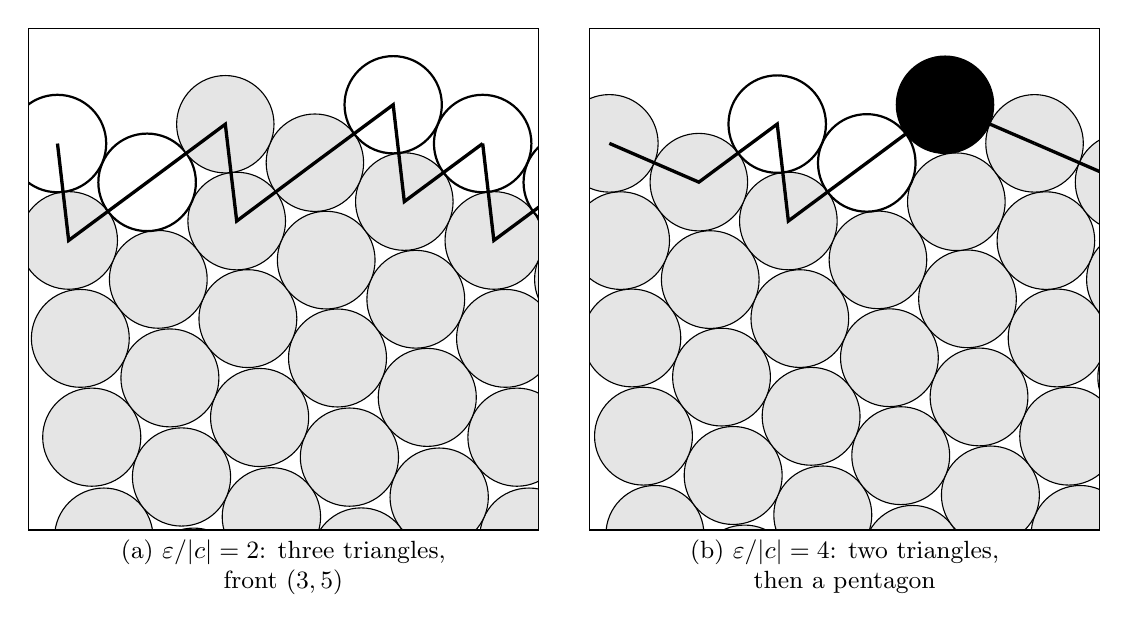
\begin{tikzpicture}[x=5.4cm,y=5.4cm]
\begin{scope}\clip (0,0) rectangle (1.2,1.18);
% generated by verify/pattern_figure.py (clean)
\draw[fill=black!10] (0.6005,-0.2067) circle (0.1160);
\draw[fill=black!10] (0.9944,-0.1587) circle (0.1159);
\draw[fill=black!10] (0.3892,-0.1114) circle (0.1158);
\draw[fill=black!10] (1.3892,-0.1114) circle (0.1158);
\draw[fill=black!10] (0.7830,-0.0639) circle (0.1158);
\draw[fill=black!10] (0.1777,-0.0171) circle (0.1157);
\draw[fill=black!10] (1.1777,-0.0171) circle (0.1157);
\draw[fill=black!10] (0.5719,0.0308) circle (0.1157);
\draw[fill=black!10] (0.9665,0.0771) circle (0.1156);
\draw[fill=black!10] (0.3605,0.1246) circle (0.1155);
\draw[fill=black!10] (1.3605,0.1246) circle (0.1155);
\draw[fill=black!10] (0.7554,0.1713) circle (0.1155);
\draw[fill=black!10] (0.1494,0.2182) circle (0.1154);
\draw[fill=black!10] (1.1494,0.2182) circle (0.1154);
\draw[fill=black!10] (0.5442,0.2645) circle (0.1154);
\draw[fill=black!10] (1.5442,0.2645) circle (0.1154);
\draw[fill=black!10] (0.9385,0.3118) circle (0.1153);
\draw[fill=black!10] (0.3332,0.3576) circle (0.1152);
\draw[fill=black!10] (1.3332,0.3576) circle (0.1152);
\draw[fill=black!10] (0.7274,0.4044) circle (0.1152);
\draw[fill=black!10] (0.1225,0.4506) circle (0.1151);
\draw[fill=black!10] (1.1225,0.4506) circle (0.1151);
\draw[fill=black!10] (0.5166,0.4970) circle (0.1151);
\draw[fill=black!10] (1.5166,0.4970) circle (0.1151);
\draw[fill=black!10] (0.9115,0.5426) circle (0.1150);
\draw[fill=black!10] (0.3059,0.5894) circle (0.1150);
\draw[fill=black!10] (1.3059,0.5894) circle (0.1150);
\draw[fill=black!10] (0.7008,0.6346) circle (0.1149);
\draw[fill=black!10] (0.0951,0.6809) circle (0.1148);
\draw[fill=black!10] (1.0951,0.6809) circle (0.1148);
\draw[fill=black!10] (0.4903,0.7265) circle (0.1148);
\draw[fill=black!10] (1.4903,0.7265) circle (0.1148);
\draw[fill=black!10] (0.8845,0.7723) circle (0.1147);
\draw[fill=white,thick] (0.2796,0.8175) circle (0.1147);
\draw[fill=white,thick] (1.2796,0.8175) circle (0.1147);
\draw[fill=black!10] (0.6742,0.8637) circle (0.1146);
\draw[fill=white,thick] (0.0688,0.9088) circle (0.1146);
\draw[fill=white,thick] (1.0688,0.9088) circle (0.1146);
\draw[fill=black!10] (0.4635,0.9542) circle (0.1145);
\draw[fill=black!10] (1.4635,0.9542) circle (0.1145);
\draw[fill=white,thick] (0.8583,1.0000) circle (0.1144);
\draw[very thick] (0.0688,0.9088) -- (0.0951,0.6809) -- (0.2796,0.8175) -- (0.4635,0.9542) -- (0.4903,0.7265) -- (0.6742,0.8637) -- (0.8583,1.0000) -- (0.8845,0.7723) -- (1.0688,0.9088);
\draw[very thick] (1.0688,0.9088) -- (1.0951,0.6809) -- (1.2796,0.8175) -- (1.4635,0.9542) -- (1.4903,0.7265) -- (1.6742,0.8637) -- (1.8583,1.0000) -- (1.8845,0.7723) -- (2.0688,0.9088);
\end{scope}
\draw (0,0) rectangle (1.2,1.18);
\node[below,font=\small,align=center] at (0.6,0) {(a) $\eps/|c|=2$: three triangles,\\front $(3,5)$};
\begin{scope}[shift={(1.32,0)}]\clip (0,0) rectangle (1.2,1.18);
% generated by verify/pattern_figure.py (break)
\draw[fill=black!10] (0.5758,-0.1969) circle (0.1154);
\draw[fill=black!10] (0.9707,-0.1507) circle (0.1153);
\draw[fill=black!10] (0.3648,-0.1038) circle (0.1153);
\draw[fill=black!10] (1.3648,-0.1038) circle (0.1153);
\draw[fill=black!10] (0.7597,-0.0576) circle (0.1153);
\draw[fill=black!10] (0.1539,-0.0106) circle (0.1152);
\draw[fill=black!10] (1.1539,-0.0106) circle (0.1152);
\draw[fill=black!10] (0.5487,0.0352) circle (0.1152);
\draw[fill=black!10] (1.5487,0.0352) circle (0.1152);
\draw[fill=black!10] (0.9429,0.0822) circle (0.1152);
\draw[fill=black!10] (0.3379,0.1281) circle (0.1152);
\draw[fill=black!10] (1.3379,0.1281) circle (0.1152);
\draw[fill=black!10] (0.7320,0.1747) circle (0.1151);
\draw[fill=black!10] (0.1270,0.2206) circle (0.1151);
\draw[fill=black!10] (1.1270,0.2206) circle (0.1151);
\draw[fill=black!10] (0.5212,0.2673) circle (0.1151);
\draw[fill=black!10] (1.5212,0.2673) circle (0.1151);
\draw[fill=black!10] (0.9161,0.3128) circle (0.1150);
\draw[fill=black!10] (0.3105,0.3595) circle (0.1150);
\draw[fill=black!10] (1.3105,0.3595) circle (0.1150);
\draw[fill=black!10] (0.7054,0.4051) circle (0.1150);
\draw[fill=black!10] (0.0997,0.4515) circle (0.1150);
\draw[fill=black!10] (1.0997,0.4515) circle (0.1150);
\draw[fill=black!10] (0.4947,0.4971) circle (0.1149);
\draw[fill=black!10] (1.4947,0.4971) circle (0.1149);
\draw[fill=black!10] (0.8890,0.5435) circle (0.1149);
\draw[fill=black!10] (0.2840,0.5888) circle (0.1149);
\draw[fill=black!10] (1.2840,0.5888) circle (0.1149);
\draw[fill=black!10] (0.6784,0.6352) circle (0.1148);
\draw[fill=black!10] (0.0734,0.6805) circle (0.1148);
\draw[fill=black!10] (1.0734,0.6805) circle (0.1148);
\draw[fill=black!10] (0.4677,0.7266) circle (0.1148);
\draw[fill=black!10] (1.4677,0.7266) circle (0.1148);
\draw[fill=black!10] (0.8628,0.7719) circle (0.1148);
\draw[fill=black!10] (0.2572,0.8180) circle (0.1147);
\draw[fill=black!10] (1.2572,0.8180) circle (0.1147);
\draw[fill=white,thick] (0.6521,0.8632) circle (0.1147);
\draw[fill=black!10] (0.0467,0.9092) circle (0.1147);
\draw[fill=black!10] (1.0467,0.9092) circle (0.1147);
\draw[fill=white,thick] (0.4415,0.9545) circle (0.1146);
\draw[fill=white,thick] (1.4415,0.9545) circle (0.1146);
\draw[fill=black] (0.8361,1.0000) circle (0.1146);
\draw[very thick] (0.0467,0.9092) -- (0.2572,0.8180) -- (0.4415,0.9545) -- (0.4677,0.7266) -- (0.6521,0.8632) -- (0.8361,1.0000) -- (1.0467,0.9092);
\draw[very thick] (1.0467,0.9092) -- (1.2572,0.8180) -- (1.4415,0.9545) -- (1.4677,0.7266) -- (1.6521,0.8632) -- (1.8361,1.0000) -- (2.0467,0.9092);
\end{scope}
\begin{scope}[shift={(1.32,0)}]\draw (0,0) rectangle (1.2,1.18);
\node[below,font=\small,align=center] at (0.6,0) {(b) $\eps/|c|=4$: two triangles,\\then a pentagon};\end{scope}
\end{tikzpicture}
\caption{The top of the stack at the end of step two, for the first two runs of Table~\ref{tab:example}
($\beta=0.523$, $\eps=0.005$, $c=-0.0025$ and $-0.00125$), drawn from the simulator (\texttt{verify/pattern\_figure.py}). The cylinder
is unrolled, with circumference $1$, and a little more than one turn is shown. Open disks are the triangle
transitions of step two, the black disk is the pentagon, and the thick line is the front. In (a) the
front ends with $5$ up vectors; in (b) the pentagon removes one again.}\label{fig:pattern}
\end{figure}

\subsection*{Results} Our main result is an immediate obstruction. We then examine how the
same local geometry can reappear after a long rhombic phase.

The immediate failure happens at hexagonal fronts. A rhombic lattice front whose notch hinge is exactly
$60^\circ$ is a piece of the hexagonal packing, and it exists for every $(m,n)$ with $m,n\ge2$ and
$n/2<m<2n$ (Lemma~\ref{lem:notch60}); its up vectors have bearing $u$ with $\tan u=\sqrt3m/(2n-m)$. Write
$H(\alpha,\sigma,\eps,c)$ for the same front with three hinges changed by small amounts, $180^\circ+\alpha$
between the last two down vectors, $60^\circ+\sigma$ at the notch and $180^\circ-\eps$ between the first two up
vectors, the ridge taking up the difference, and with every disk, the initial ones included, of
diameter~\eqref{eq:diam} (Definition~\ref{def:hexfront}). Put $\kappa_u=\cos(u-60^\circ)$.

\begin{theorem}[Pentagon on the first disk]\label{thm:static}
Let $m,n\ge2$ with $n/2<m<2n$, and let $a,s,e$ and $q>0$ satisfy
\begin{equation}\label{eq:window}
\max\Bigl(e-a+\frac q2\kappa_u,\;-\frac q2\kappa_u\Bigr)\;<\;s\;<\;e-\frac q4\bigl(\sqrt3\sin u+5\cos u\bigr).
\end{equation}
Then for all sufficiently small $t>0$, $H(ta,ts,te,-tq)$ is a valid front and the first disk placed on it is
a pentagon.
\end{theorem}

\noindent The two lower bounds say only that no two disks of the front overlap, at the ridge and at the
notch (Lemma~\ref{lem:valid}). The upper bound is the real condition: the pentagon disk must clear its
neighbour. All three hold, for example, when $e>0$, $a=e/2$, $s=3e/4$ and $0<q\le e/20$. For $(2,3)$, $\kappa_u=5/(2\sqrt7)$ and
the upper bound is $s<e-\tfrac{13\sqrt7}{28}q$.
The rate enters with a sign: shrinking pushes the pentagon disk onto its neighbour, so a pentagon needs the
rate to be small compared with the mismatch. Along such a ray both directional deviations are $O(t)$ and the product irregularity is
$O(t^2)$; see~\eqref{eq:irregularity}. Thus the construction also applies when both vector
families are required to be nearly regular.

\begin{corollary}[No independent tolerance box]\label{cor:GDD}
Fix $m,n\ge2$ with $n/2<m<2n$. For every $\eps_1,\eps_2,\eps_3>0$, there is a valid front
with both directional deviations below $\eps_1$, notch angle below $60^\circ+\eps_2$, and
rate below $\eps_3$, whose first placement is a pentagon.
\end{corollary}

\begin{proof}
Take $(a,s,e,q)=(\tfrac12,\tfrac34,1,\tfrac1{20})$ in Theorem~\ref{thm:static}.
The two directional deviations tend to zero with $t$, the notch angle is $60^\circ+3t/4$,
and the rate is $t/20$. Choose $t>0$ small enough to satisfy all three prescribed bounds
and the conclusion of the theorem.
\end{proof}

\subsection*{Relation to the constant-diameter classification}
Gol\'e and Douady~\cite{GD} work at constant diameter. They classify the offspring of every notch
with at most three vectors by its hinge angles and one bearing~\cite[Sec.~4]{GD}, and use this
classification to prove that stacking from any cylindrical chain with parastichy numbers $(1,2)$ or
$(2,1)$ converges to a rhombic tiling~\cite[Thm.~1]{GD}. Their reduction from a whole front to its
short notches is proved for the chains that arise there~\cite[Props.~4.4, 4.5]{GD}; for longer
chains they give simulations and heuristic arguments~\cite[Sec.~2.4]{GD}.
Theorem~\ref{thm:static} overlaps with their work in exactly one place. At $q=0$ the disks $A,B,C,E$
form a notch with one down and two up vectors, with hinges $\tau=60^\circ+\sigma$ and
$\gamma=180^\circ-\eps$, and their pentagon condition $\gamma+\tau\le240^\circ$ reads $\sigma\le\eps$,
the zero-rate form of the upper bound in~\eqref{eq:window}. Three things are new.
\begin{enumerate}
\item \emph{The whole periodic front.} Near a hexagonal front, the lowest site is not decided inside
one short notch. Six parent pairs meet at it, including $Z$ and $E$, which lie two diameters apart
across a notch with two down and two up vectors, and the result has to hold for every $(m,n)$ with
$m,n\ge2$. Lemma~\ref{lem:hexsite} and the proof of Theorem~\ref{thm:static} settle this
degenerate site and exclude every other site of the front.
\item \emph{The rate.} Shrinking moves the pentagon boundary by $-\tfrac q4(\sqrt3\sin u+5\cos u)$, so it
works against the pentagon. It also closes the ridge, so the hexagonal front is no longer valid once
$c<0$; every valid front near it carries a second irregularity (Lemma~\ref{lem:valid}). The window
compares the mismatch with the rate on the same scale. It is a first-disk counterpart of the ratio
law described below.
\item \emph{The conjecture.} The tolerance conjecture of~\cite{GDD} requires $c<0$, and it is not
treated in~\cite{GD}. Corollary~\ref{cor:GDD} alone could also be obtained from the case $q=0$ of the
whole-front argument, by perturbing $c$ at fixed $t$; item~1 is needed either way. The first-order rate
term adds how small the rate must be: below a fixed multiple of the mismatch.
\end{enumerate}

\noindent This obstruction uses fronts whose notch excess is smaller than their directional mismatch.
Requiring the mismatch to be small relative to the initial notch excess excludes this particular
construction. The three-disk family below tests whether that protection survives later
transitions: each slow triangle leaves a notch excess on the much smaller scale $|c|$, while the
cancellation estimate allows an initial mismatch to persist.

\subsection*{The delayed mechanism} For this we study a three-disk family. Write $F(\beta,\eps)$ for the $(1,2)$ front of the example
(Definition~\ref{def:front}), with $\beta$ in the interval $(\beta_{\min},\pi/6)$,
$\beta_{\min}=\arctan(-\sqrt3/2)+\pi/3\approx19.107^\circ$, on which it is a valid front that has not yet
reached a triangle transition. Its notch angle exceeds $60^\circ$ by an amount fixed by $\beta$, far more
than its irregularity, so Theorem~\ref{thm:static} does not apply to it.

\begin{theorem}[First transition]\label{thm:A}
For every $\beta\in(\beta_{\min},\pi/6)$ there are $\eps_0,c_0>0$ such that for $|\eps|<\eps_0$ and
$-c_0<c<0$, stacking from $F(\beta,\eps)$ performs two triangle transitions, on different up
vectors, and no pentagon transition before its front first has parastichy numbers $(3,2)$.
\end{theorem}

\noindent Theorem~\ref{thm:A} is the first step of the delayed mechanism; its main tool is the
cancellation estimate of Proposition~\ref{prop:frozen}, which carries the mismatch $\eps$ through
long rhombic phases with an error of order $|c|$. Whether the inherited mismatch later produces a
pentagon, between $(3,2)$ and $(8,5)$, is not proved here. An exact first-order event calculation and
the simulations support it, and we state it as Conjecture~\ref{thm:B} in Section~\ref{sec:steptwo},
together with what a proof still needs. Nothing in Theorems~\ref{thm:static} and~\ref{thm:A} or
Corollary~\ref{cor:GDD} depends on it.

The numerics in Section~\ref{sec:numerics} locate the threshold for $F(\beta,\eps)$. Over thirty starting
angles $\beta\in[0.40,0.52]$ and three rates, none of the sampled second transitions breaks at sampled ratios $\eps/|c|\le2.3$, and
all break at sampled ratios $\eps/|c|\ge3.4$ (Figure~\ref{fig:pr}). We refer to this empirical crossover as the
\emph{ratio law}; it is not a monotonicity theorem or a universal threshold. Gol\'e, Dumais and Douady observed that irregularity alone drives the pattern towards
quasi-symmetry~\cite[p.~29, item (iii)]{GDD}, and Swinton found that noise and rate ``interact in a complex
way''~\cite[Sec.~5.3]{Swinton2024} and noted that there is no theoretical guidance on the critical
rate~\cite[Sec.~6]{Swinton2024}. The ratio law is a quantitative form
of that interaction for one initial irregularity.

\subsection*{The geometric mechanism} Figure~\ref{fig:pent} shows the relevant local geometry. A triangle transition at a slow rate is nearly equilateral, so it leaves a notch whose hinge is
$60^\circ$ plus a cushion of order $|c|$ (Lemma~\ref{lem:triangle}). During the long rhombic phases
between transitions the shape of the front is frozen to first order (Proposition~\ref{prop:frozen}),
so an initial mismatch $\eps$ between the up vectors is retained up to $O(|c|)$ over a
phase of length $O(1/|c|)$. When two mismatched up vectors
meet a $60^\circ$ notch, a pentagon fits once the mismatch beats the cushion (Lemma~\ref{lem:pent}).
Slower growth reduces the local clearance scale. Establishing that this necessarily selects
a pentagon later in the three-disk dynamics is the remaining issue in Conjecture~\ref{thm:B}.

\subsection*{Plan} Section~\ref{sec:model} sets up the model. Section~\ref{sec:first} gives the first-order
rhombus and triangle steps, and Section~\ref{sec:static} uses them to prove Theorem~\ref{thm:static}.
Section~\ref{sec:frozen} proves that front shape is frozen through rhombic phases. Section~\ref{sec:stepone}
proves Theorem~\ref{thm:A}; Section~\ref{sec:steptwo} develops the evidence for
Conjecture~\ref{thm:B}. Section~\ref{sec:numerics}
reports the ratio law and Section~\ref{sec:discussion} discusses a narrower conjecture and open problems.

\section{The model}\label{sec:model}

\subsection{Disks, fronts and transitions}
Work on the cylinder $\R/\Lambda\mathbb Z\times\R$, identified with a strip of the complex plane, with
height $y=\Imag z$. A disk centred at $z$ has diameter
\begin{equation}\label{eq:diam}
d(z)=b_0+c\,\Imag z,\qquad c<0,
\end{equation}
so disks placed higher are smaller, and $|c|$ is the rate of decrease per unit of height (the rate
of~\cite{GDD}). Two disks touch when the distance between their centres is the mean of their
diameters. Each new disk is placed at the lowest admissible position above the front where it touches
two front disks and overlaps no disk, including periodic images~\cite{GDD,GD}. Only positions with
positive diameter are considered. The transition statements concern this upper placement branch;
contacts below the front do not define placements.

A \emph{front} is a closed chain of disks $z_0,z_1,\dots,z_{N-1}$ winding once around the cylinder,
consecutive disks touching, on top of the stack~\cite{AtelaGole,GD}. Its \emph{front vectors} are
$v_k=z_{k+1}-z_k$, read from left to right. A vector pointing down ($\Imag v_k<0$) is a \emph{down
vector}; the others are \emph{up vectors}, following the convention that a horizontal vector is
up~\cite{GDD}. We write $(m,n)$ for the numbers of down and up vectors; these are the parastichy
numbers of the front. The \emph{hinge} at $z_{k+1}$ is the upper angle between the two vectors,
\begin{equation}\label{eq:hinge}
h(v_k,v_{k+1})=\arg v_k+\pi-\arg v_{k+1},
\end{equation}
read as: the angle above the chain at the joint. A \emph{notch} is a down vector followed by an up
vector. Its hinge is the notch angle $\eta$ of~\cite{GDD}; in bearing angles,
$\eta=\pi-(\arg U-\arg D)$. Figure~\ref{fig:front} shows the smallest example, the front with one down
and two up vectors used throughout this paper.

\begin{figure}[t]
\centering
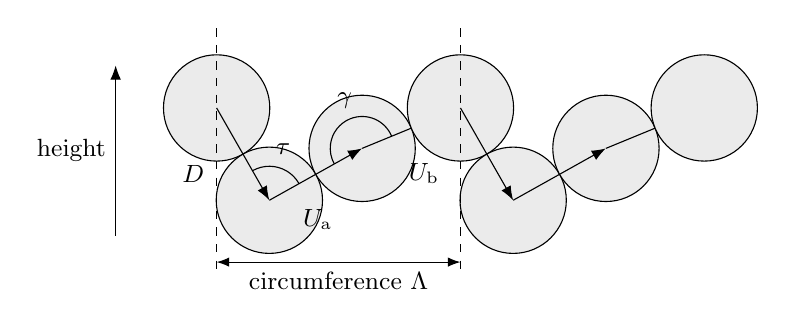
\begin{tikzpicture}[x=1.35cm,y=1.35cm,every node/.style={font=\small}]
% front F(beta, eps) with beta = 0.45, eps = 0.12 (exaggerated), unit diameters; coordinates from
% z1 = D, z2 = D + Ua, z3 = D + Ua + Ub = (Lambda, 0) with Lambda = 2.2936 (computed in verify/schematic note)
\foreach \s in {0,2.2936} {
  \foreach \x/\y in {0/0,0.4959/-0.8684,1.3687/-0.3802} \draw[fill=black!8] (\x+\s,\y) circle (0.5);
  \draw[-{Latex[length=1.8mm]}] ($(0,0)+(\s,0)$)--($(0.4959,-0.8684)+(\s,0)$);
  \draw[-{Latex[length=1.8mm]}] ($(0.4959,-0.8684)+(\s,0)$)--($(1.3687,-0.3802)+(\s,0)$);
  \draw[-{Latex[length=1.8mm]}] ($(1.3687,-0.3802)+(\s,0)$)--($(2.2936,0)+(\s,0)$);
}
\draw[fill=black!8] (4.5872,0) circle (0.5);
\node at (-0.22,-0.62) {$D$};
\node at (0.95,-1.05) {$U_{\mathrm a}$};
\node at (1.95,-0.62) {$U_{\mathrm b}$};
\draw (0.4959,-0.8684) ++(29.2:0.32) arc (29.2:119.7:0.32);
\node at ($(0.4959,-0.8684)+(75:0.5)$) {$\tau$};
\draw (1.3687,-0.3802) ++(22.3:0.3) arc (22.3:209.2:0.3);
\node at ($(1.3687,-0.3802)+(110:0.48)$) {$\gamma$};
\draw[dashed] (0,0.75)--(0,-1.55); \draw[dashed] (2.2936,0.75)--(2.2936,-1.55);
\draw[{Latex[length=1.6mm]}-{Latex[length=1.6mm]}] (0,-1.45)--node[below]{circumference $\Lambda$} (2.2936,-1.45);
\draw[-{Latex[length=1.8mm]}] (-0.95,-1.2)--node[left]{height} (-0.95,0.4);

\end{tikzpicture}
\caption{The front $F(\beta,\eps)$ of Definition~\ref{def:front}, two turns of the unrolled cylinder,
with the up-vector mismatch $\eps$ exaggerated. It has one down vector $D$ and two up vectors, so its
parastichy numbers are $(1,2)$. The notch hinge $\tau$ sits between $D$ and $\Ua$; the hinge $\gamma$
between the two up vectors differs from $180^\circ$ by $\eps$.}\label{fig:front}
\end{figure}

For the up and down vector families, define their complex means $\mu_U$, $\mu_D$ and deviations
\begin{equation}\label{eq:irregularity}
\eta_U=\frac{\max_j|U_j-\mu_U|}{|\mu_U|},\qquad
\eta_D=\frac{\max_k|D_k-\mu_D|}{|\mu_D|},\qquad
I=\eta_U\eta_D,\qquad J=\max(\eta_U,\eta_D).
\end{equation}
The means are nonzero for the fronts considered here. The irregularity of~\cite{GDD} is the
product $I$. We also record $J$, which controls both directional deviations separately.
For a single down vector $\eta_D=0$, so $I=0$ even when the up vectors differ. The first-disk
construction has $J\to0$ as well as $I\to0$ and does not rely on this degeneracy.

A new disk touching $z_a$ and $z_b$ replaces the disks strictly between them in the front. There are
three cases (Figure~\ref{fig:transitions}):
\begin{itemize}
\item \emph{triangle} (T): $b=a+1$. One vector is replaced by two; the front gains a vector.
\item \emph{rhombus} (R): $b=a+2$. A notch $D,U$ is replaced by $U',D'$; the vector count is kept.
\item \emph{pentagon} (P): $b=a+3$. Three vectors are replaced by two; the front loses a vector.
\end{itemize}
At constant diameter, Gol\'e and Douady classified the offspring of notches by their hinge angles. A
notch with one down and one up vector gives a rhombus when its hinge lies in $[\pi/3,2\pi/3]$ and a
triangle, resting on the less steep of its two vectors, when the hinge lies in $[2\pi/3,\pi]$. A notch
$D,U_1,U_2$ can give a pentagon only when its two hinges $\tau=h(D,U_1)$ and $\gamma=h(U_1,U_2)$ satisfy
$\gamma+\tau\le4\pi/3$~\cite[Prop.~4.3]{GD}.

\begin{figure}[t]
\centering
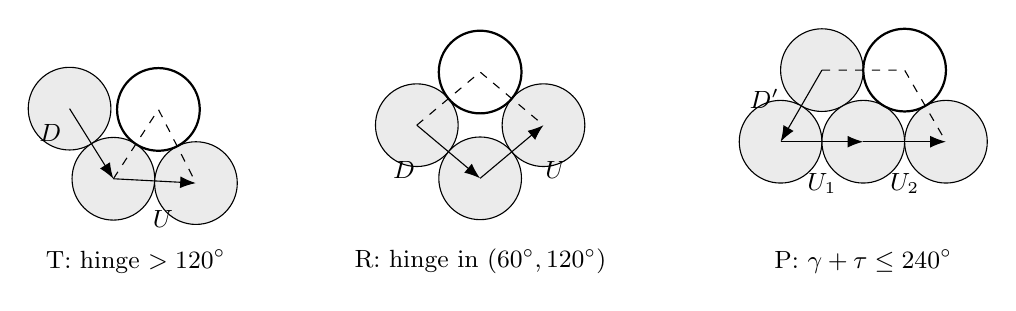
\begin{tikzpicture}[scale=1.05,every node/.style={font=\small}]
\begin{scope}
\foreach \p in {(0,0),(0.5299,-0.8480),(1.5285,-0.9004)} \draw[fill=black!8] \p circle (0.5);
\draw[thick] (1.0746,-0.0094) circle (0.5);
\draw[-{Latex[length=2mm]}] (0,0)--(0.5299,-0.8480) node[pos=0.35,left=5pt] {$D$};
\draw[-{Latex[length=2mm]}] (0.5299,-0.8480)--(1.5285,-0.9004) node[pos=0.6,below=7pt] {$U$};
\draw[dashed] (0.5299,-0.8480)--(1.0746,-0.0094)--(1.5285,-0.9004);
\node at (0.8,-1.85) {T: hinge $>120^\circ$};
\end{scope}
\begin{scope}[xshift=4.2cm,yshift=-0.2cm]
\foreach \p in {(0,0),(0.7660,-0.6428),(1.5321,0)} \draw[fill=black!8] \p circle (0.5);
\draw[thick] (0.7660,0.6428) circle (0.5);
\draw[-{Latex[length=2mm]}] (0,0)--(0.7660,-0.6428) node[pos=0.3,below left=4pt] {$D$};
\draw[-{Latex[length=2mm]}] (0.7660,-0.6428)--(1.5321,0) node[pos=0.7,below right=4pt] {$U$};
\draw[dashed] (0,0)--(0.7660,0.6428)--(1.5321,0);
\node at (0.77,-1.65) {R: hinge in $(60^\circ,120^\circ)$};
\end{scope}
\begin{scope}[xshift=8.6cm,yshift=-0.4cm]
\foreach \p in {(0.5,0.8660),(0,0),(1,0),(2,0)} \draw[fill=black!8] \p circle (0.5);
\draw[thick] (1.5,0.8660) circle (0.5);
\draw[-{Latex[length=2mm]}] (0.5,0.8660)--(0,0) node[pos=0.4,left=6pt] {$D'$};
\draw[-{Latex[length=2mm]}] (0,0)--(1,0) node[pos=0.5,below=8pt] {$U_1$};
\draw[-{Latex[length=2mm]}] (1,0)--(2,0) node[pos=0.5,below=8pt] {$U_2$};
\draw[dashed] (0.5,0.8660)--(1.5,0.8660)--(2,0);
\node at (1,-1.45) {P: $\gamma+\tau\le240^\circ$};
\end{scope}
\end{tikzpicture}
\caption{The three transitions. Grey disks belong to the front, the open disk is new, and dashed
segments join it to the two disks it touches. The pentagon panel is drawn at the degenerate point
$\gamma+\tau=240^\circ$, where the new disk touches all three of $P_0$, $P_2$, $P_3$
(Lemma~\ref{lem:pent}).}\label{fig:transitions}
\end{figure}

\subsection{The initial fronts}
\begin{definition}\label{def:front}
For $\beta\in(\beta_{\min},\pi/6)$ and small $\eps$, the front $F(\beta,\eps)$ consists of three touching
disks whose diameters follow~\eqref{eq:diam}, with front vectors $D,\Ua,\Ub$, where $\arg\Ua=\beta+\eps/2$,
$\arg\Ub=\beta-\eps/2$ and $D$ is the down vector closing the chain:
$\Imag(D+\Ua+\Ub)=0$. The circumference is $\Lambda=\Real(D+\Ua+\Ub)$.
\end{definition}

\noindent At $c=0$ all three disks have diameter $b_0$. One could instead give the initial disks a common
diameter, treating the first front as data outside the law~\eqref{eq:diam}; that changes the front by
$O(|c|)$. The analytic first-transition argument is stable under this change, but it shifts the measured threshold of the ratio law
(Section~\ref{sec:numerics}), because a defect of order $|c|$ is itself an irregularity on the scale that
matters.

So $\Ua$ is the steeper up vector when $\eps>0$. For $\eps=c=0$ this is the $(1,2)$ rhombic lattice with
$\sin\beta_D=-2\sin\beta$, and its notch angle is $\pi-\beta+\beta_D$, which decreases to $60^\circ$ as
$\beta\to\pi/6$ (it is $62.6^\circ$ at $\beta=0.523$). At $\beta=\beta_{\min}$ the notch angle is
$120^\circ$ and the front is already at its triangle threshold (Lemma~\ref{lem:threshold}).

A \emph{Fibonacci transition} from a front with $(m,n)$, $n$ up vectors, is a sequence of $n$ triangle
transitions, one on each up vector, with rhombic phases in between and no pentagon, ending at
$(m+n,n)$; the next one exchanges the roles of up and down vectors. This is the scenario of~\cite[p.~25]{GDD}.
From $F(\beta,\eps)$ the first Fibonacci transition is $(1,2)\to(2,2)\to(3,2)$ and the second is
$(3,2)\to(3,3)\to(3,4)\to(3,5)$.

\subsection{Limiting tilings}\label{sec:tilings} Three configurations at constant diameter organise the
proofs, because the slow dynamics stays close to them: the $(1,2)$ lattice at its triangle threshold, the
$(2,2)$ front it leaves after one triangle, and the tiling $K_0$ reached from the $(3,2)$ lattice at its
threshold after two triangles of step two. At a threshold the up vectors are exactly $60^\circ$ above the
down vectors, so that a notch hinge equals $120^\circ$.

\begin{lemma}[Threshold law]\label{lem:threshold}
A rhombic lattice front with $m$ down vectors of angle $\beta_D$ and $n$ up vectors of angle
$\beta_D+\pi/3$ closes, that is $m\sin\beta_D+n\sin(\beta_D+\pi/3)=0$, if and only if
\[
\tan\beta_D=-\frac{\sqrt3\,n}{2m+n}.
\]
For $(m,n)=(1,2)$ this gives $\tan\beta_D=-\sqrt3/2$, $\beta_D\approx-40.893^\circ$, up angle
$\beta_{\min}\approx19.107^\circ$. For $(m,n)=(3,2)$ it gives $\tan\beta_D=-\sqrt3/4$,
$\beta_D\approx-23.413^\circ$, up angle $36.587^\circ$.
\end{lemma}

\noindent In words: the more down vectors per up vector, the flatter the down vectors are when the
first triangle becomes possible.

\begin{proof}
Expand $\sin(\beta_D+\pi/3)=\tfrac12\sin\beta_D+\tfrac{\sqrt3}2\cos\beta_D$: the closing condition
becomes $(2m+n)\sin\beta_D+\sqrt3\,n\cos\beta_D=0$.
\end{proof}

Both thresholds are independent of $\beta$ and $\eps$. This is why the constants below are universal:
the starting angle only sets how long the slow drift takes to reach them. A convenient exact model:
in units of the diameter, the $(3,2)$ threshold vectors are
\begin{equation}\label{eq:K0vectors}
D=\tfrac{1}{\sqrt{19}}(4,-\sqrt3),\quad U=\tfrac{1}{2\sqrt{19}}(7,3\sqrt3),\quad
S=\tfrac{1}{2\sqrt{19}}(1,-5\sqrt3),
\end{equation}
with $U$ and $S$ the rotations of $D$ by $+60^\circ$ and $-60^\circ$. Writing points as
$(X/\sqrt{19},\sqrt3\,Y/\sqrt{19})$ makes every point of these tilings rational in $(X,Y)$, and
squared distances equal $(\Delta X^2+3\Delta Y^2)/19$. All distances quoted for the tiling $K_0$ below
are exact rational identities in this model; the $(1,2)$ threshold works the same way with $7$ in place
of $19$. These identities are checked in Lean (\lean{Tilings.lean}).

\begin{table}[h]
\centering\small
\begin{tabular}{@{}ll@{}}
\toprule
$c<0$, $b_0$ & rate of decrease of the diameter, diameter at height $0$\\
$\beta$, $\eps$ & mean angle and mismatch of the two up vectors of $F(\beta,\eps)$\\
$D$, $U$; $\beta_D$, $\beta_U$ & down and up vectors and their bearing angles\\
$\Ua$, $\Ub$; $U^{+}$, $U^{-}$ & the two up vectors; the up and down vectors a triangle on $U$ creates\\
$h$, $\tau$, $\gamma$ & hinge~\eqref{eq:hinge}; notch hinge; hinge between two up vectors\\
$\omega$ & $e^{i\pi/3}$, rotation by $60^\circ$\\
$\sigma$, $\delta$ & cushion above $60^\circ$ after a triangle; overshoot of a hinge past $120^\circ$\\
$\theta$ & mismatch between the two up vectors of a pentagon notch\\
$\kappa_1$, $\kappa_2$ & loss of mismatch through step one; pentagon correction (Lemma~\ref{lem:pent})\\
$K_0$, $K^*$ & limiting tiling at the pentagon (Lemma~\ref{lem:K0}); measured threshold of $\eps/|c|$\\
\bottomrule
\end{tabular}
\caption{Notation.}\label{tab:notation}
\end{table}

\section{First-order transitions}\label{sec:first}

Rhombic phases last about $1/|c|$ steps, so a uniform error of order $c^2$ per step contributes order $|c|$ over such a phase.
This makes uniform local estimates essential. This section computes them.

\subsection{The apex branch} Fix a notch, let the rate $c$ vary, and keep the disks of the notch
touching their neighbours. The new disk is a transversal intersection of two tangency conditions, so
it moves smoothly with $c$.

\begin{lemma}[Apex branch]\label{lem:apex}
Let $A(c)$ and $C(c)$ be $C^1$ families of centres and let $q_0$ satisfy $|q_0-A(0)|=|q_0-C(0)|=b_0$
with $q_0-A(0)$ and $q_0-C(0)$ not parallel. Then there is a unique $C^1$ family $Q(c)$ near $c=0$ with
$Q(0)=q_0$ such that the disk at $Q(c)$ touches the disks at $A(c)$ and $C(c)$ under~\eqref{eq:diam}.
\end{lemma}

\begin{proof}
The two tangency conditions $|Q-A|^2=(b_0+c(\Imag A+\Imag Q)/2)^2$ and the same with $C$ define a $C^1$
map of $(c,Q)$ whose partial derivative in $Q$ at $(0,q_0)$ is
$v\mapsto\bigl(2(q_0-A)\cdot v,\;2(q_0-C)\cdot v\bigr)$, which is invertible exactly when the two
contact normals are not parallel. The implicit function theorem gives $Q$.
\end{proof}

Differentiating one tangency condition at $c=0$, where all diameters equal $b_0$, gives the identity
used in every proof below:
\begin{equation}\label{eq:tangency}
(Q-P)\cdot(Q'-P')=\tfrac{b_0}{2}\,(\Imag P+\Imag Q).
\end{equation}
In words: the rate at which the gap between two touching disks opens equals the rate at which their
mean diameter grows, which at $c=0$ is half the sum of their heights times $b_0$.

\subsection{The rhombus step}
\begin{figure}[t]
\centering
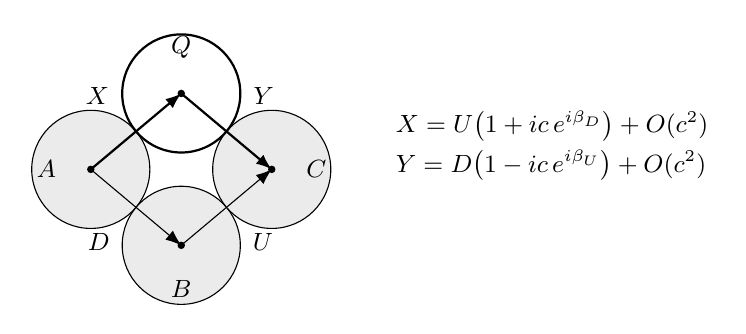
\begin{tikzpicture}[scale=1.5,every node/.style={font=\small}]
\coordinate (A) at (0,0); \coordinate (B) at (0.7660,-0.6428); \coordinate (C) at (1.5321,0);
\coordinate (Q) at (0.7660,0.6428);
\foreach \p in {A,B,C} \draw[fill=black!8] (\p) circle (0.5);
\draw[thick] (Q) circle (0.5);
\draw[-{Latex[length=2mm]}] (A)--(B) node[pos=0.5,below left=6pt] {$D$};
\draw[-{Latex[length=2mm]}] (B)--(C) node[pos=0.5,below right=6pt] {$U$};
\draw[-{Latex[length=2mm]},thick] (A)--(Q) node[pos=0.5,above left=6pt] {$X$};
\draw[-{Latex[length=2mm]},thick] (Q)--(C) node[pos=0.5,above right=6pt] {$Y$};
\foreach \p in {A,B,C,Q} \fill (\p) circle (0.9pt);
\node[left=9pt] at (A) {$A$}; \node[below=9pt] at (B) {$B$}; \node[right=9pt] at (C) {$C$}; \node[above=9pt] at (Q) {$Q$};
\node[align=left,anchor=west] at (2.5,0.2) {$X=U\bigl(1+ic\,e^{i\beta_D}\bigr)+O(c^2)$\\[2pt]
$Y=D\bigl(1-ic\,e^{i\beta_U}\bigr)+O(c^2)$};
\end{tikzpicture}
\caption{A rhombus step. At $c=0$ the new cell is the rhombus $X=U$, $Y=D$; with shrinking disks
each new vector is the old one turned and stretched by a factor that depends only on the other
vector of the notch (Lemma~\ref{lem:rhombus}).}\label{fig:rhombus}
\end{figure}

\begin{lemma}[Rhombus step]\label{lem:rhombus}
Let $A\xrightarrow{D}B\xrightarrow{U}C$ be a notch of touching disks with $D$ and $U$ not parallel,
and let $Q$ be the apex branch touching $A$ and $C$ with $Q=A+U$ at $c=0$. Put $X=Q-A$, $Y=C-Q$ and
$\xi=X-U$. Then
\[
\xi'(0)=\frac{i\,UD}{b_0}\quad\text{(complex product)},
\]
so that, with $D=b_0e^{i\beta_D}$ and $U=b_0e^{i\beta_U}$,
\[
X=U\bigl(1+ic\,e^{i\beta_D}\bigr)+O(c^2),\qquad Y=D\bigl(1-ic\,e^{i\beta_U}\bigr)+O(c^2).
\]
\end{lemma}

The formula says that the up vector is multiplied by a factor that depends only on the down vector it
passes, and the down vector by a factor that depends only on the up vector. Proposition~\ref{prop:frozen}
is built on that.

\begin{proof}
Apply~\eqref{eq:tangency} to the four touching pairs $AB$, $BC$, $AQ$, $QC$. At $c=0$, $Q-A=U$ and
$C-Q=D$, and the heights satisfy $\Imag Q=\Imag A+\Imag U$, $\Imag C=\Imag B+\Imag U$. Subtracting the
equations for $BC$ from $AQ$, and $QC$ from $AB$, the unknown motions of $A,B,C$ cancel and
\[
U\cdot\xi'=-b_0\Imag D,\qquad D\cdot\xi'=-b_0\Imag U.
\]
This $2\times2$ system has a unique solution because $U$ and $D$ are not parallel, and
$\xi'=iUD/b_0$ satisfies it: with $|U|=|D|=b_0$, $U\cdot(iUD)/b_0=\Real(\bar U\,iUD)/b_0=-b_0\Imag D$,
and similarly for $D$.
\end{proof}

\subsection{The triangle step and the cushion}
\begin{lemma}[Triangle step]\label{lem:triangle}
Let $B\xrightarrow{U}C$ be touching disks and $Q$ the apex branch touching both with $Q=B+\omega U$
at $c=0$, where $\omega=e^{i\pi/3}$. Put $X=Q-B$, $Y=C-Q$ and $\xi=X-\omega U$. Then
\[
\xi'(0)=\frac{i\,U^2}{2b_0},\qquad\text{so}\qquad X=\omega U+\tfrac{ic}{2}e^{i\beta_U}U+O(c^2),\quad
Y=\bar\omega U-\tfrac{ic}{2}e^{i\beta_U}U+O(c^2).
\]
Consequently, to first order in $c$:
\begin{enumerate}
\item[(a)] $\arg X-\arg(\omega U)=\tfrac c2\cos(\beta_U-\pi/3)$;
\item[(b)] $\arg X-\arg Y=\tfrac{2\pi}3+\tfrac c2\cos\beta_U$.
\end{enumerate}
If the triangle fires on the up vector of a notch whose hinge is $120^\circ+\delta$, the new notch at $B$
has hinge
\begin{equation}\label{eq:cushion}
60^\circ+\delta+\tfrac{|c|}{2}\cos(\beta_U-60^\circ)+O(c^2).
\end{equation}
\end{lemma}

\begin{proof}
The three tangencies $BC$, $BQ$, $QC$ and~\eqref{eq:tangency} give, after the same cancellation as before,
$(\omega U)\cdot\xi'=\tfrac{b_0}2\Imag(\omega U-U)$ and $(\bar\omega U)\cdot\xi'=-\tfrac{b_0}2\Imag(\omega U)$,
whose unique solution is $iU^2/(2b_0)$. For (a), $X/(\omega U)=1+\xi/(\omega U)$ and the derivative of its
argument is $\Imag\bigl(iU/(2b_0\omega)\bigr)=\tfrac12\cos(\beta_U-\pi/3)$; (b) adds the same computation for
$Y/(\bar\omega U)$, using $\cos(\beta-\pi/3)+\cos(\beta+\pi/3)=\cos\beta$. The new hinge at $B$ is
$h(D,X)=h(D,U)-(\arg X-\arg U)=120^\circ+\delta-60^\circ-\tfrac c2\cos(\beta_U-60^\circ)$, and $c<0$.
\end{proof}

At $c=0$ and $\delta=0$ the new hinge is exactly $60^\circ$: the new disk touches the disk below $B$ as
well. That triple contact is the pentagon boundary, and~\eqref{eq:cushion} measures how far a slow
triangle stays from it. The cushion is of order $|c|$; the overshoot $\delta$ is also of order $|c|$,
since hinges drift by order $|c|$ per step (Corollary~\ref{cor:rates}).

\begin{corollary}[Rotation rates]\label{cor:rates}
In the rhombus step of Lemma~\ref{lem:rhombus}, to first order in $c$,
$\arg X-\arg U=c\cos\beta_D$ and $\arg Y-\arg D=-c\cos\beta_U$.
\end{corollary}

\begin{proof}
$X/U=1+\xi/U$ and $\Imag(\xi'/U)=\Imag(iD/b_0)=\cos\beta_D$; likewise $Y/D=1-\xi/D$.
\end{proof}

\subsection{Uniform remainders}
The derivative identities above hold for $C^1$ input families. A rhombic phase applies them about
$1/|c|$ times, so it needs an $O(c^2)$ remainder that is uniform over all notches met along the way;
$C^1$ regularity alone does not give that. Two observations supply it.

First, the law has no preferred scale. Translate a disk $B$ of diameter $b$ to the origin and divide
all lengths by $b$. The law becomes $d=1+cy$ with the same dimensionless slope $c$, since $c$ is a
ratio of a change in diameter to a change in height. Second, edge lengths are explicit. An edge of
bearing $\beta$ leaving a disk of diameter $b$ ends at a disk of diameter $b+c\ell\sin\beta$, so
tangency, $\ell=b+\tfrac c2\ell\sin\beta$, gives
\begin{equation}\label{eq:edge-exact}
\ell=\frac{b}{1-\frac c2\sin\beta}.
\end{equation}

\begin{lemma}[Uniform remainders]\label{lem:uniform}
Let $\mathcal K$ be a compact set of bearing pairs $(\beta_D,\beta_U)$ with $\beta_U-\beta_D\notin\pi\mathbb Z$.
There are $c_1>0$ and $R$ such that for every notch $A\xrightarrow{D}B\xrightarrow{U}C$ of touching disks
with bearings in $\mathcal K$, whatever the diameter $b$ of $B$, and every $|c|\le c_1$, the rhombus apex
exists and
\[
\frac XU=1+ic\,e^{i\beta_D}+r_X,\qquad \frac YD=1-ic\,e^{i\beta_U}+r_Y,\qquad |r_X|,|r_Y|\le Rc^2.
\]
The same holds for the triangle step of Lemma~\ref{lem:triangle} over any compact set of bearings
$\beta_U$, and for any apex whose two contact normals at $c=0$ are not parallel.
\end{lemma}

\begin{proof}
By scale invariance take $B=0$ and $b=1$. By~\eqref{eq:edge-exact},
\[
A=-\frac{e^{i\beta_D}}{1+\frac c2\sin\beta_D},\qquad C=\frac{e^{i\beta_U}}{1-\frac c2\sin\beta_U},
\]
which are real-analytic in $p=(\beta_D,\beta_U,c)$ for $|c|<2$. The apex $Q$ solves $\Phi(Q,p)=0$, where
\[
\Phi(Q,p)=\Bigl(|Q-A|^2-\tfrac14(d_A+d_Q)^2,\;|Q-C|^2-\tfrac14(d_C+d_Q)^2\Bigr),\qquad d_Q=1+c\Imag Q,
\]
is polynomial in $Q$, $A$, $C$ and $c$, hence real-analytic. At $c=0$ the solution is
$Q_*(\beta)=A+e^{i\beta_U}$, and the derivative of $\Phi$ in $Q$ there is
$v\mapsto2\bigl((Q_*-A)\cdot v,(Q_*-C)\cdot v\bigr)$, with determinant $\pm4\sin(\beta_U-\beta_D)$. This is
bounded away from zero on $\mathcal K$.

The analytic implicit function theorem gives, around each point $(\beta,0)$ with $\beta\in\mathcal K$, a
neighbourhood and a radius $\rho_\beta$ such that $\Phi(Q,p)=0$ has exactly one solution with
$|Q-Q_*(\beta)|<\rho_\beta$, depending analytically on $p$. Finitely many of these neighbourhoods cover
$\mathcal K\times\{0\}$. Where two overlap, the two solutions agree by uniqueness, provided they lie within
the smaller radius, and this holds after shrinking the neighbourhoods, because $Q_*$ is uniformly
continuous. So there are $c_1>0$ and one analytic branch $Q(\beta,c)$ on a neighbourhood of
$\mathcal K\times[-c_1,c_1]$.

The quotient $f=X/U=(Q-A)/C$ is analytic there, since $|C|\ge\tfrac12$. Taylor's theorem in $c$ at fixed
$\beta$, applied to the real and imaginary parts, gives
\[
f(\beta,c)=f(\beta,0)+c\,\partial_cf(\beta,0)+r_X,\qquad |r_X|\le c^2\sup_{\mathcal K\times[-c_1,c_1]}|\partial_c^2f|.
\]
The supremum is finite by compactness. Here $f(\beta,0)=1$, and Lemma~\ref{lem:rhombus}, applied to the
family with fixed bearings, gives $\partial_cf(\beta,0)=ie^{i\beta_D}$. The same argument applies to
$Y/D=(C-Q)/(-A)$. For the triangle step, the normals $\omega U$ and $\bar\omega U$ are never parallel, so
any compact set of $\beta_U$ works. The last sentence is the same argument with the corresponding
$Q_*$.
\end{proof}

\noindent The coefficients are evaluated at the bearings current at each step, not at the initial
ones. The analytic and compactness argument is not formalised in Lean.

\section{The first disk near a hexagonal front}\label{sec:static}

A rhombic lattice front whose notch hinge is exactly $60^\circ$ is a piece of the hexagonal packing:
every disk of the front touches its neighbours in the triangular lattice. This section shows that such
fronts are unstable in the direction the conjecture cares about. Perturb a few hinges by amounts of
order $t$ and let the disks shrink at a rate of order $t$, and the very first disk can be a pentagon.

\subsection{The notch-60 lattice}
\begin{lemma}[Notch-60 law]\label{lem:notch60}
A rhombic lattice front with $m$ down vectors and $n$ up vectors of bearing $u$, the down vectors at
$u-120^\circ$ (notch hinge $60^\circ$), closes if and only if
\[
\tan u=\frac{\sqrt3\,m}{2n-m}.
\]
Both families point to the right, $30^\circ<u<90^\circ$, exactly when $n/2<m<2n$.
\end{lemma}

\begin{proof}
Expand $\sin(u-2\pi/3)=-\tfrac12\sin u-\tfrac{\sqrt3}2\cos u$: the closing condition
$m\sin(u-2\pi/3)+n\sin u=0$ becomes $(2n-m)\sin u=\sqrt3\,m\cos u$. The bounds on $u$ are $\tan u>1/\sqrt3$
and $2n-m>0$.
\end{proof}

\noindent For $(2,3)$ this gives $\tan u=\sqrt3/2$, $u\approx40.89^\circ$ and down bearing
$\approx-79.11^\circ$; for $(1,2)$ it gives a vertical down vector, which is why the construction below
needs $m,n\ge2$.

\begin{definition}\label{def:hexfront}
Let $m,n\ge2$ with $n/2<m<2n$. Write the front word as $D_1\cdots D_m\,U_1\cdots U_n$ and name the disks
around the notch $Z\xrightarrow{D_{m-1}}A\xrightarrow{D_m}B\xrightarrow{U_1}C\xrightarrow{U_2}E$. The front
$H(\alpha,\sigma,\eps,c)$ has all its disks, the seeds included, of diameter~\eqref{eq:diam}, consecutive disks
touching, and the hinges of the notch-60 lattice except four:
\begin{gather*}
h(D_{m-1},D_m)=180^\circ+\alpha,\qquad h(D_m,U_1)=60^\circ+\sigma,\qquad h(U_1,U_2)=180^\circ-\eps,\\
h(U_n,D_1)=300^\circ-(\alpha+\sigma-\eps).
\end{gather*}
\end{definition}

The last hinge, at the ridge, is forced: the deviations $h-180^\circ$ of the hinges of a closed front sum
to zero. To fix scale and vertical translation, set the diameter of the first disk to $1$ at height $0$.
The bearings have the form $\phi+\beta_j(\alpha,\sigma,\eps)$, where the hinges determine the relative
bearings $\beta_j$. Generate the edge lengths by~\eqref{eq:edge-exact}. At zero parameters the
vertical closing error has derivative $\sum_j\cos\beta_j=\Lambda_0>0$ with respect to $\phi$.
The implicit function theorem therefore determines an analytic closing rotation for small
parameters. Horizontal closure defines the positive circumference. The last tangency is included
in this recurrence, since its endpoint returns to height $0$ and hence to diameter $1$.
Both $\eta_U$ and $\eta_D$ are $O(|\alpha|+|\eps|+|c|)$, so their maximum has this bound and
their product has its square as a bound. The one notch angle is
$60^\circ+\sigma$, and the rate is $|c|$.

At $t=0$ the disks of $H$ sit on the triangular lattice $\{xD+yU:x,y\in\mathbb Z\}$, where $D$ and $U$ now
denote the unit down and up vectors. Since $D\cdot U=-\tfrac12$,
\begin{equation}\label{eq:eisenstein}
|xD+yU|^2=x^2-xy+y^2,
\end{equation}
which takes the values $0,1,3,4,7,\dots$ and never $2$. Two disks of $H$ that are not neighbours are at
distance at least $\sqrt3$ at $t=0$, except two pairs at distance $1$: the disks on either side of the
notch, $A$ and $C$, and the disks on either side of the ridge. Indeed, going right from one disk to the
other along the front adds the vectors of a proper cyclic subword of $D^mU^n$, with sum $xD+yU$,
$0\le x\le m$, $0\le y\le n$. By~\eqref{eq:eisenstein} this has length $1$ only for $(x,y)$ equal to
$(1,0)$ or $(0,1)$, which are neighbours, or $(1,1)$, which is the subword $DU$ at the notch or $UD$ at
the ridge. The other images of the second disk add $k(mD+nU)$. For $k=-1$ the result is minus the sum
of the complementary subword, covered by the same list. For $k\ge1$ or $k\le-2$ both coordinates are
at least $2$ or both at most $-2$, and since $x^2-xy+y^2=\tfrac14(x+y)^2+\tfrac34(x-y)^2$ the squared
length is at least $4$.

\begin{lemma}[Validity]\label{lem:valid}
Along $(\alpha,\sigma,\eps,c)=t(a,s,e,-q)$ the clearances of these two pairs are, to first order,
$\tfrac{\sqrt3}2\bigl(s+\tfrac q2\kappa_u\bigr)t$ at the notch and $\tfrac{\sqrt3}2\bigl(a+s-e-\tfrac q2\kappa_u\bigr)t$ at the
ridge, with $\kappa_u=\cos(u-60^\circ)$. So the lower bounds in~\eqref{eq:window} make $H(ta,ts,te,-tq)$ a
valid front for small $t>0$.
\end{lemma}

\begin{proof}
Let $T$ be the middle disk of either triple and $L$, $R$ its neighbours. Write $\ell_1=|T-L|$,
$\ell_2=|T-R|$, and let $\phi$ be the angle of the triangle $LTR$ at $T$: the angle above the chain at the
notch and below it at the ridge. Then $\phi$ is $60^\circ$ plus a hinge deviation, which the
definition prescribes exactly: $\phi=60^\circ+\sigma$ at the notch and $\phi=60^\circ+(\alpha+\sigma-\eps)$ at the
ridge. By the law of cosines,
\[
|L-R|^2=\ell_1^2+\ell_2^2-2\ell_1\ell_2\cos\phi .
\]
At $t=0$, $\ell_1=\ell_2=|L-R|=1$ and $\phi=60^\circ$, so
$\tfrac{d}{dt}|L-R|=\tfrac12(\dot\ell_1+\dot\ell_2)+\tfrac{\sqrt3}2\dot\phi$. Tangency gives
$\ell_1=\tfrac12(d_T+d_L)$ and $\ell_2=\tfrac12(d_T+d_R)$ exactly. The clearance of the pair is
$g=|L-R|-\tfrac12(d_L+d_R)$, so
\[
\dot g=\tfrac{\sqrt3}2\dot\phi+\tfrac12\Bigl(\dot d_T-\tfrac12(\dot d_L+\dot d_R)\Bigr).
\]
With $c=-qt$ and heights $y_k$ at $t=0$, $\dot d_k=-q\,(y_k-y_0)$, and the reference height $y_0$ cancels.
At the ridge $T$ is reached by $U_n$ and left by $D_1$, so
$y_T-\tfrac12(y_L+y_R)=\tfrac12(\Imag U-\Imag D)=\tfrac12\bigl(\sin u-\sin(u-120^\circ)\bigr)=\tfrac{\sqrt3}2\kappa_u$; at the
notch the same expression is $-\tfrac{\sqrt3}2\kappa_u$. Hence
\[
\dot g_{\mathrm{notch}}=\tfrac{\sqrt3}2\bigl(s+\tfrac q2\kappa_u\bigr),\qquad
\dot g_{\mathrm{ridge}}=\tfrac{\sqrt3}2\bigl(a+s-e-\tfrac q2\kappa_u\bigr).
\]
Every other pair of non-neighbours is at distance at least $\sqrt3$ at $t=0$, by the remark before the
lemma, so it stays clear for small $t$. Neighbours touch by construction. Under the lower bounds
in~\eqref{eq:window} both derivatives are positive, so $g>0$ at both pairs for small $t>0$.
\end{proof}

\noindent Shrinking closes the ridge: the hexagonal front itself is not a valid front once $c<0$, and the
ridge has to open by at least $\tfrac q2\kappa_u t$. With the other hinges at their lattice values this forces
$\alpha+\sigma-\eps>0$, so with $\sigma<\eps$ the down vectors must be irregular too ($a>0$). On fronts with
$m+n\ge5$ one can instead perturb another hinge inside a run, which changes nothing at $Q_0$.

Theorem~\ref{thm:static} of the introduction says that $H(ta,ts,te,-tq)$ places a pentagon first when
$(a,s,e,q)$ satisfies~\eqref{eq:window}. The rest of this section proves it.

\subsection{The lowest site}
\begin{figure}[t]
\centering
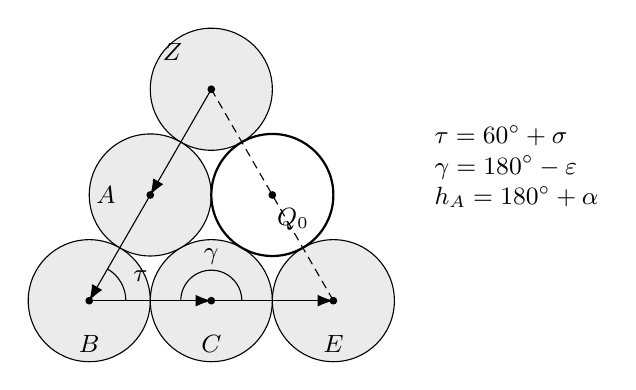
\begin{tikzpicture}[scale=1.55,every node/.style={font=\small}]
\coordinate (Z) at (1,1.7321); \coordinate (A) at (0.5,0.8660); \coordinate (B) at (0,0);
\coordinate (C) at (1,0); \coordinate (E) at (2,0); \coordinate (Q) at (1.5,0.8660);
\foreach \p in {Z,A,B,C,E} \draw[fill=black!8] (\p) circle (0.5);
\draw[thick] (Q) circle (0.5);
\foreach \p in {Z,A,B,C,E,Q} \fill (\p) circle (0.9pt);
\draw[-{Latex[length=2mm]}] (Z)--(A); \draw[-{Latex[length=2mm]}] (A)--(B);
\draw[-{Latex[length=2mm]}] (B)--(C); \draw[-{Latex[length=2mm]}] (C)--(E);
\draw[densely dashed] (Z)--(E);
\node[above left=7pt] at (Z) {$Z$}; \node[left=9pt] at (A) {$A$}; \node[below=9pt] at (B) {$B$};
\node[below=9pt] at (C) {$C$}; \node[below=9pt] at (E) {$E$}; \node at ($(Q)+(0.17,-0.2)$) {$Q_0$};
\draw (0.3,0) arc (0:60:0.3); \node at (0.42,0.2) {$\tau$};
\draw (1.25,0) arc (0:180:0.25); \node at (1,0.36) {$\gamma$};
\node[align=left,anchor=west] at (2.75,1.1) {$\tau=60^\circ+\sigma$\\$\gamma=180^\circ-\eps$\\$h_A=180^\circ+\alpha$};
\end{tikzpicture}
\caption{The notch of a hexagonal front, turned so that $U_1=C-B$ is horizontal. The site $Q_0$ touches
four front disks, $Z$, $A$, $C$ and $E$, and $Z$, $E$ are two diameters apart (dashed). The pentagon disk
touches $A$ and $E$; at constant diameter it must clear $C$, which needs $\eps>\sigma$, and fit between $Z$
and $E$, which needs $2\sigma+\alpha>\eps$.}\label{fig:hex}
\end{figure}

\begin{lemma}\label{lem:hexsite}
At $\alpha=\sigma=\eps=c=0$, with unit diameters:
\begin{enumerate}
\item[(a)] every position touching two front disks is a lattice point;
\item[(b)] among lattice points strictly above the front, the lowest are $Q_0=A+U$ and its periodic
images, and every other one is higher by at least $\min(|\Imag D|,\Imag U)$;
\item[(c)] $Q_0$ touches exactly the four front disks $Z,A,C,E$; $|Z-E|=2$ with $Q_0$ the midpoint, and
$|Q_0-B|=\sqrt3$.
\end{enumerate}
\end{lemma}

\begin{proof}
(a) A position touching disks at $P$ and $R$ has $|Q-P|=|Q-R|=1$, so $|P-R|\le2$, and
by~\eqref{eq:eisenstein} $|P-R|$ is $1$, $\sqrt3$ or $2$. The lattice is invariant under rotation by
$60^\circ$. In the first case $Q=P+(R-P)e^{\pm i\pi/3}$. In the second, the six solutions
of $x^2-xy+y^2=3$ show that $R-P=w+we^{i\pi/3}$ for a unit lattice vector $w$, and the two positions are
$P+w$ and $P+we^{i\pi/3}$. In the third, the solutions of $x^2-xy+y^2=4$ are twice the unit vectors, and
$Q$ is the midpoint. In each case $Q$ is a lattice point.

(b) Use coordinates $xD+yU$ and put $\delta=-\Imag D>0$, $\upsilon=\Imag U>0$. The height is
$-x\delta+y\upsilon$, and closure of the period $mD+nU$ gives $m\delta=n\upsilon$. Take $B$ as the origin and
$A=(-1,0)$, so the front vertices are $(x,0)$ for $-m\le x\le0$ and $(0,y)$ for $0\le y\le n$, repeated
with period $(m,n)$. The map $(x,y)\mapsto xD+yU$ preserves orientation and $\Real D,\Real U>0$, so the front is a
graph over the horizontal axis, and a point lies above it exactly when it lies to the left of the
staircase traversed in the direction of increasing $x$ and $y$. Write a lattice point as
$(km-j,\,y)$ with $k\in\mathbb Z$ and $1\le j\le m$. It is strictly above the front exactly when
$y\ge kn+1$. Relative to $B$, and using $km\delta=kn\upsilon$, its height is
\[
-(km-j)\delta+y\upsilon=j\delta+(y-kn)\upsilon\;\ge\;j\delta+\upsilon .
\]
This is smallest, $\delta+\upsilon$, exactly for $j=1$, $y=kn+1$, which is
$(-1,1)+k(m,n)=Q_0+k(mD+nU)$. Any other point has $j\ge2$ or $y\ge kn+2$, and so is higher by at least
$\delta$ or $\upsilon$.

(c) The six unit neighbours of $Q_0=(-1,1)$ are $Q_0+(1,0)=(0,1)=C$, $Q_0-(0,1)=A$,
$Q_0+(1,1)=(0,2)=E$, $Q_0-(1,1)=(-2,0)=Z$, and $(-1,2)$, $(-2,1)$. The last two are not front vertices,
because $m,n\ge2$. Then $Z-E=-2(D+U)$ has length $2$ with midpoint $Q_0$, and $Q_0-B=U-D$ has length
$\sqrt3$ by~\eqref{eq:eisenstein}.
\end{proof}

\noindent So six pairs share the apex $Q_0$: $ZA$ (a triangle on $D_{m-1}$), $AC$ (the rhombus), $CE$ (a
triangle on $U_2$), $AE$ and $ZC$ (pentagons) and $ZE$ (a transition removing three vectors). The first
disk is decided among them at first order. The pair $ZE$ is degenerate and is treated by
its separation, rather than by a transverse-apex expansion.

\subsection{First-order clearances}
Turn and translate the configuration so that $B=0$ and $U_1$ points along $1$; clearances do not change,
and the height enters only multiplied by $c$, so its first-order change does not matter. Then
$A=\omega$, $C=1$, $E=2$, $Z=2\omega$, $Q_0=1+\omega$ with $\omega=e^{i\pi/3}$, and the contact normals
$n_k=Q_0-z_k$ are
\[
n_A=1,\qquad n_C=\omega,\qquad n_E=\omega-1,\qquad n_Z=1-\omega.
\]
Along $(\alpha,\sigma,\eps,c)=t(a,s,e,-q)$ write $\dot z$ for $dz/dt$ at $t=0$. For a candidate family $Q(t)=Q_0+t x+o(t)$, differentiating the clearance $|Q-z_k|-\tfrac12(d_k+d_Q)$ as in~\eqref{eq:tangency} shows that, to
first order, the disk is clear of $z_k$ to strict first order when $n_k\cdot x>\lambda_k$; a tangency requires $n_k\cdot x=\lambda_k$, with
\[
\lambda_k=n_k\cdot\dot z_k-\tfrac q2\,h_k
\]
and $h_k$ the height of $z_k$ above $Q_0$ (diameters normalised to $1$ at the height of $Q_0$).

\begin{lemma}\label{lem:hexclear}
Put $\mu_C=\lambda_A+\lambda_E-\lambda_C$ and $\mu_Z=-(\lambda_Z+\lambda_E)$. To first order:
\begin{enumerate}
\item[(a)] the disk touching $A$ and $E$ clears $C$ by $\mu_C$ and $Z$ by $\mu_Z$;
\item[(b)] the disks touching $A,C$ and $C,E$ overlap $E$ and $A$ by $\mu_C$, and the disk touching $Z,C$
overlaps $A$ by $\mu_C+\mu_Z$;
\item[(c)] if $\mu_Z>0$ no disk near $Q_0$ touches both $Z$ and $E$, and the disk touching $Z,A$ is higher than the one
touching $A,E$ by $\tfrac2{\sqrt3}\mu_Z\cos u$;
\item[(d)] $\mu_C=\tfrac{\sqrt3}2(e-s)-\tfrac q8\bigl(3\sin u+5\sqrt3\cos u\bigr)$ and
$\mu_Z=\tfrac{\sqrt3}2(2s+a-e)+\tfrac q2\bigl(3\sin u+\sqrt3\cos u\bigr)$, per unit $t$.
\end{enumerate}
\end{lemma}

\begin{proof}
Parts (a) to (c) use only $n_E=n_C-n_A$ and $n_Z=-n_E$. At the vertex $n_A\cdot x=\lambda_A$, $n_E\cdot x=\lambda_E$ one gets
$n_C\cdot x-\lambda_C=\lambda_A+\lambda_E-\lambda_C$ and $n_Z\cdot x-\lambda_Z=-\lambda_E-\lambda_Z$. At $n_A\cdot x=\lambda_A$, $n_C\cdot x=\lambda_C$ the
clearance to $E$ is $\lambda_C-\lambda_A-\lambda_E=-\mu_C$, and symmetrically for $C,E$ against $A$. At $n_Z\cdot x=\lambda_Z$,
$n_C\cdot x=\lambda_C$ the clearance to $A$ is $\lambda_Z+\lambda_C-\lambda_A=-\mu_C-\mu_Z$.

The pair $ZE$ has opposite normals, so it has no transverse apex and needs a separate argument. Suppose
a disk at $Q$ touches both, with $Q\to Q_0$ as $t\to0$. By the triangle inequality
\[
|Z-E|\le|Q-Z|+|Q-E|=\tfrac12(d_Z+d_E)+d_Q,
\]
so $g(t)=|Z-E|-\tfrac12(d_Z+d_E)-d_Q\le0$. Normalise diameters to $1$ at the height of $Q_0$ at $t=0$;
then $d_Q=1+c\,(\Imag Q-\Imag Q_0)=1+o(t)$. Since $Z-E=-2n_Z$ with $|n_Z|=1$ at $t=0$,
\[
g(t)=t\bigl(-n_Z\cdot\dot Z-n_E\cdot\dot E+\tfrac q2(h_Z+h_E)\bigr)+o(t)=t\,\mu_Z+o(t),
\]
using $n_E=-n_Z$ and $\dot d_k=-qh_k$. So $\mu_Z>0$ gives $g(t)>0$ for small $t>0$, a contradiction. No
apex expansion is used, so this covers candidates whose distance from $Q_0$ is much larger than $t$.
The vertices $ZA$ and $AE$ both lie on
the line $n_A\cdot x=\lambda_A$, a distance $\tfrac2{\sqrt3}\mu_Z$ apart along $in_A$, whose height in the cylinder
frame is $\cos u>0$.

(d) The hinges give $\dot A=is\,\omega$, $\dot C=0$, $\dot E=ie$, $\dot Z=i(2s+a)\omega$ at $q=0$, so
$\lambda_A=-\tfrac{\sqrt3}2s$, $\lambda_C=0$, $\lambda_E=\tfrac{\sqrt3}2e$ and $\lambda_Z=-\tfrac{\sqrt3}2(2s+a)$. The rate stretches
each side to the mean of its two diameters, adding $-q\ell_{BC}$ to $\dot C$, $-q(\ell_{BC}+\ell_{CE})$ to $\dot E$,
$-q\ell_{AB}\omega$ to $\dot A$ and $-q(\ell_{AB}+\ell_{ZA})\omega$ to $\dot Z$, where $\ell_{XY}=\tfrac12(h_X+h_Y)$.
Collecting terms,
\[
\mu_C^{q}=-\tfrac q4\,(3h_A-h_B-5h_C+h_E),\qquad \mu_Z^{q}=-\tfrac q4\,(2h_A+2h_B+2h_C-h_Z-h_E),
\]
and the heights are $h_z=-\Imag\bigl(e^{iu}(Q_0-z)\bigr)$: $h_A=-\sin u$, $h_B=-\sqrt3\sin(u+30^\circ)$,
$h_C=-\sin(u+60^\circ)$, $h_E=-\sin(u+120^\circ)$, $h_Z=-\sin(u-60^\circ)$. Since
$\sin(u-60^\circ)+\sin(u+120^\circ)=0$ this gives (d).
\end{proof}

\begin{proof}[Proof of Theorem~\ref{thm:static}]
By Lemma~\ref{lem:valid} the front is valid for small $t>0$. By~(d) the upper bound in~\eqref{eq:window} is
$\mu_C>0$. Since $\tfrac12(3\sin u+\sqrt3\cos u)=\sqrt3\kappa_u$, (d) and Lemma~\ref{lem:valid} give $\mu_Z$ as the sum
of the notch and ridge clearance rates plus $\sqrt3q\kappa_u$, so $\mu_Z>0$ on every valid front.

\emph{The pentagon disk is a valid position.} The normals $n_A$ and $n_E$ are not parallel, so
Lemma~\ref{lem:apex} gives a $C^1$ family $Q_{AE}(t)\to Q_0$ touching $A$ and $E$. By
Lemma~\ref{lem:hexclear}(a) its clearances from $C$ and $Z$ are $t\mu_C+o(t)$ and $t\mu_Z+o(t)$, both
positive for small $t$. Every other front disk, periodic images included, is at distance at least
$\sqrt3$ from $Q_0$ at $t=0$ (Lemma~\ref{lem:hexsite}(c) and~\eqref{eq:eisenstein}), so it stays clear.
$Q_0$ is strictly above the front, and the front moves continuously with $t$, so $Q_{AE}(t)$ is above it.

\emph{Nothing else is as low.} Suppose that for some sequence $t_k\to0$ there is a valid position
$Q_k\ne Q_{AE}(t_k)$ with $\Imag Q_k\le\Imag Q_{AE}(t_k)$, touching front disks $P_k$ and $R_k$. We derive a
contradiction in three steps.

\smallskip\noindent\emph{Step 1: compactness.} Normalise the diameter to $1$ at height $0$, so the front
disks have diameters in $[\tfrac12,2]$ and heights in a fixed bounded interval for small $t$. If $Q$ touches
$P$, then $|\Imag Q-\Imag P|\le|Q-P|=d_P+\tfrac c2(\Imag Q-\Imag P)$, so $|\Imag Q-\Imag P|\le2d_P\le4$ once $|c|\le\tfrac12$.
Hence $Q_k$ has bounded height, and modulo the period it lies in a bounded set. Its parents lie within
distance $4$ of it, and the circumference is bounded below, so up to periodic translation $P_k$ and
$R_k$ range over a finite set of front disks and images. Passing to a subsequence, the pair
$(P_k,R_k)$ is fixed and $Q_k\to Q^*$.

\smallskip\noindent\emph{Step 2: the limit is $Q_0$.} Touching and non-overlap are closed conditions, and
all diameters tend to $1$. So $Q^*$ is at distance exactly $1$ from the limits of $P_k$ and $R_k$, and at
distance at least $1$ from every front disk at $t=0$. By Lemma~\ref{lem:hexsite}(a), $Q^*$ is a lattice
point. It lies on or above the limiting front. The only lattice points on the front polyline are its
vertices, which are front disks at distance $0$, so $Q^*$ is strictly above. Finally
$\Imag Q^*\le\lim\Imag Q_{AE}(t_k)=\Imag Q_0$. By Lemma~\ref{lem:hexsite}(b), $Q^*$ is $Q_0$ up to periodic
translation, and by Lemma~\ref{lem:hexsite}(c) the limiting parents are two of $Z,A,C,E$.

\smallskip\noindent\emph{Step 3: the six pairs.} For large $k$, $Q_k$ is a position near $Q_0$ touching one
of the six pairs. Five of them have non-parallel normals at $Q_0$. For these, the implicit function
theorem in the proof of Lemma~\ref{lem:apex}, with $t$ in place of $c$, gives a neighbourhood of $Q_0$ in
which the touching position is unique for small $t$ and lies on the $C^1$ apex family, so $Q_k$ lies on
that family.
\begin{itemize}
\item $AE$: then $Q_k=Q_{AE}(t_k)$, which was excluded.
\item $AC$, $CE$ and $ZC$: by Lemma~\ref{lem:hexclear}(b) these families overlap $E$, $A$ and $A$ by
$t\mu_C+o(t)$, $t\mu_C+o(t)$ and $t(\mu_C+\mu_Z)+o(t)$, so they are not valid for large $k$.
\item $ZA$: by Lemma~\ref{lem:hexclear}(c) it is higher than $Q_{AE}$ by $\tfrac2{\sqrt3}\mu_Z\cos u\,t+o(t)>0$.
\end{itemize}
The sixth pair, $ZE$, admits no touching position near $Q_0$, by the separation argument in the proof of
Lemma~\ref{lem:hexclear}. Every case gives a contradiction. So for small $t>0$ the pentagon disk
touching $A$ and $E$ is the unique lowest valid position, and the first transition is a pentagon.
\end{proof}

\noindent Lemma~\ref{lem:hexclear}, the notch part of Lemma~\ref{lem:valid} and the step from validity to
$\mu_Z>0$ are checked in Lean (\lean{Static.lean}): the four tangencies and three hinge rates of the front
determine the first-order clearances of all six candidates and of the notch pair. The file
\lean{StaticExists.lean} constructs the local five-disk and apex families for the prescribed
rates. Periodic closure and global exclusion are supplied by the analytic arguments above.

On valid rays above the window ($\mu_C<0$), the tested fronts place a rhombus $AC$. The independent
simulator agrees with both predictions on every valid front tested: $182$ fronts over all $26$ shapes with
$2\le m\le6$, on rays inside and above the window (\texttt{verify/static\_general.py}).
A separate brute-force enumeration confirms Lemma~\ref{lem:hexsite}(b) for all $47$ shapes with
$2\le m\le8$ (\texttt{verify/static\_lattice\_order.py}).

The theorem uses the simplest perturbation. Lemma~\ref{lem:hexclear} involves only the hinges at $A$, $B$
and $C$, so on fronts with $n\ge3$ one may also turn the hinge between $U_2$ and $U_3$, and then $\alpha=0$ is
allowed: the down vectors stay exactly regular and only the up vectors carry irregularity. The channel
condition $\mu_Z>0$ is then no longer automatic. When it fails the channel between $Z$ and $E$ is closed, no
disk fits near $Q_0$, and the first disk is placed elsewhere, a triangle in all our runs
(\texttt{verify/static\_channel.py}).


\section{Front shape is frozen during rhombic phases}\label{sec:frozen}

A \emph{rhombic phase} is a run of $L$ consecutive rhombus steps. In each step an up vector passes the
down vector on its left (Figure~\ref{fig:rhombus}). Lemma~\ref{lem:rhombus} says that the factor
an up vector receives depends only on the down vector it passes. If every up vector passed every down
vector equally often and at the same times, all up vectors would receive the same product of factors,
and their ratios would not move. The bookkeeping below shows that this is true up to boundedly many
factors, whatever the phase length.

\subsection{Pass bookkeeping} Number the $n$ up vectors in their cyclic order, which never changes, and
let $g_i$ be the number of down vectors between up $i$ and up $i+1$. Let $P_i(t)$ be the number of passes
made by up $i$ in the first $t$ steps. A pass by up $k$ moves one down vector from gap $k-1$ to gap $k$,
so
\begin{equation}\label{eq:gaps}
g_i(t)=g_i(0)+P_i(t)-P_{i+1}(t).
\end{equation}

\begin{lemma}[Pass balance, lag and sweep]\label{lem:passes}
In a rhombic phase with $m$ down and $n$ up vectors:
\begin{enumerate}
\item[(a)] $|P_j(t)-P_k(t)|\le m$ for all ups $j,k$ and all $t$;
\item[(b)] if $t_{u,k}$ is the step of the $k$-th pass of up $u$, then $|nk-t_{u,k}|\le nm$;
\item[(c)] labelling the down vectors $0,\dots,m-1$ in their cyclic order, up $u$ passes down vector
$\alpha_u-k \pmod m$ at its $k$-th pass, for a fixed $\alpha_u$.
\end{enumerate}
\end{lemma}

\begin{proof}
(a) Summing~\eqref{eq:gaps} over the gaps from up $j$ to up $k$ gives $P_j-P_k$ as the change in the
number of down vectors between them, which lies in $[-m,m]$. (b) The $n$ counts sum to $t$, so by (a)
each lies within $m$ of $t/n$; apply this at $t=t_{u,k}$, where $P_u=k$. (c) Down vectors never pass
each other, so they keep their cyclic labels. Let $r_u$ be the label of the first down vector to the
right of up $u$. A pass by $u$ moves the down vector labelled $r_u-1$ to its right, so $r_u$ drops by one;
a pass by another up changes neither the order of the down vectors nor which one is first to the right
of $u$. Consistency of the labels with the gaps, $r_{i+1}=r_i+g_i$, is preserved by every pass.
\end{proof}

\subsection{The frozen-shape proposition}
\begin{proposition}\label{prop:frozen}
Consider a rhombic phase with $m$ down and $n$ up vectors in which every step obeys
Lemma~\ref{lem:rhombus} with normalised multiplicative remainder at most $Rc^2$, and in which the phase $e^{i\beta_d(t)}$ of
each down vector changes by at most $\lambda$ per step. If $|c|+Rc^2\le\tfrac12$, then for any two up
vectors $u,v$ making $K_u$ and $K_v$ passes,
\[
\Bigl|\Delta\log\frac{U_u}{U_v}\Bigr|\le|c|\bigl(3nm\,\lambda\,K_u+3m\bigr)
+(K_u+K_v)\bigl((|c|+Rc^2)^2+Rc^2\bigr),
\]
where $\Delta\log$ is the accumulated change of the logarithm (the continuous branch along the phase).
The same holds for two down vectors with $m$ and $n$ exchanged.
\end{proposition}

With $\lambda=O(|c|)$ (each vector changes by $O(c)$ in the steps that involve it) and
$K_u\le L/n+m$, the bound is $O_{m,n}(|c|+c^2L)$. For phases of length $O(1/|c|)$, every up/up and
down/down ratio of the front, angle and length, changes by $O(|c|)$. The bound needs no smallness of
the irregularity, only the compactness of Lemma~\ref{lem:uniform}.

\begin{figure}[t]
\centering
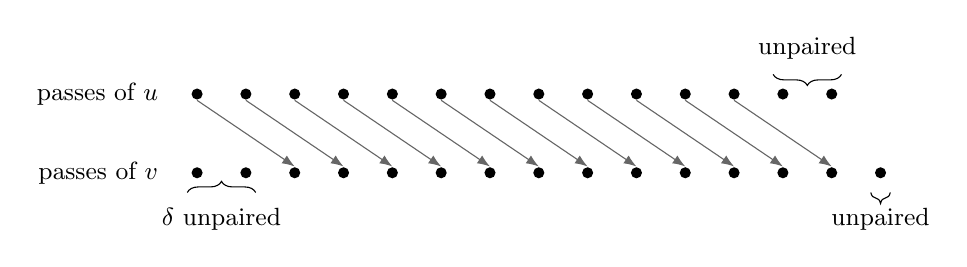
\begin{tikzpicture}[x=0.62cm,y=1cm,every node/.style={font=\small}]
\foreach \k in {0,...,13} {\fill (\k,1) circle (2pt);}
\foreach \k in {0,...,14} {\fill (\k,0) circle (2pt);}
\node[left] at (-0.6,1) {passes of $u$};
\node[left] at (-0.6,0) {passes of $v$};
\foreach \k in {0,...,11} {\draw[-{Latex[length=1.6mm]},black!60] (\k,0.92)--(\k+2,0.08);}
\draw[decorate,decoration={brace,amplitude=4pt}] (-0.2,-0.25)--node[below=2pt]{$\delta$ unpaired}(1.2,-0.25) ;
\draw[decorate,decoration={brace,amplitude=4pt}] (13.2,1.25)--node[above=2pt]{unpaired}(11.8,1.25) ;
\draw[decorate,decoration={brace,amplitude=4pt}] (14.2,-0.25)--node[below=2pt]{unpaired}(13.8,-0.25) ;
\end{tikzpicture}
\caption{The matching in the proof of Proposition~\ref{prop:frozen} with $\delta=2$. Each paired pass
meets the same down vector at times at most $3nm$ apart; at most $3m$ passes are left unpaired.}\label{fig:matching}
\end{figure}

\begin{proof}
By Lemma~\ref{lem:rhombus}, up $u$ is multiplied at its $k$-th pass by $1+ica_k+r_k$ with
$a_k=e^{i\beta_{d(u,k)}(t_{u,k})}$ and $|r_k|\le Rc^2$; likewise $1+icb_k+s_k$ for $v$. For
$|z|\le\frac12$, $|\log(1+z)-z|\le|z|^2$, so the change of $\log(U_u/U_v)$ is
$ic\bigl(\sum_{k<K_u}a_k-\sum_{k<K_v}b_k\bigr)$ up to the second term of the bound.

By Lemma~\ref{lem:passes}(c), the $k$-th pass of $u$ and the $(k+\delta)$-th pass of $v$ meet the same
down vector, where $\delta=(\alpha_v-\alpha_u)\bmod m<m$. Pair them (Figure~\ref{fig:matching}). By
(b), their times differ by at most $nm+nm+n\delta\le3nm$, so the paired phases differ by at most
$3nm\,\lambda$. Write
\[
\sum_{k<K_u}a_k-\sum_{k<K_v}b_k=\sum_{k<K}(a_k-b_{k+\delta})+\sum_{K\le k<K_u}a_k
-\sum_{j<\delta}b_j-\sum_{K+\delta\le j<K_v}b_j,
\]
with $K=\min(K_u,K_v-\delta)$. The first sum is at most $3nm\,\lambda K_u$. The other three contain
$(K_u-K)+\delta+(K_v-K-\delta)\le|K_u-K_v|+2\delta\le3m$ terms of modulus one, by (a). If
$K_v<\delta$, every term is unpaired and there are $K_u+K_v<3m$ of them.
\end{proof}

This matching proof is simpler than the cycle-by-cycle regrouping one might first try: it needs one
shift, by the offset $\delta$ of the two sweeps, and no complete cycles. Atela and Gol\'e showed that at
constant diameter the tangential eigenvalues of the stacking map at a rhombic tiling are roots of
unity~\cite{AtelaGole}, so a priori a slow forcing could build up resonantly over a phase.
Proposition~\ref{prop:frozen} shows that the first-order forcing cancels instead.

\section{The first transition}\label{sec:stepone}

Figure~\ref{fig:stepone} shows the whole first transition at its limit, $\eps=c=0$: a triangle on one up
vector, a $(2,2)$ phase in which one triple of disks comes close to a pentagon without reaching it, and a
triangle on the other up vector.

\begin{figure}[t]
\centering
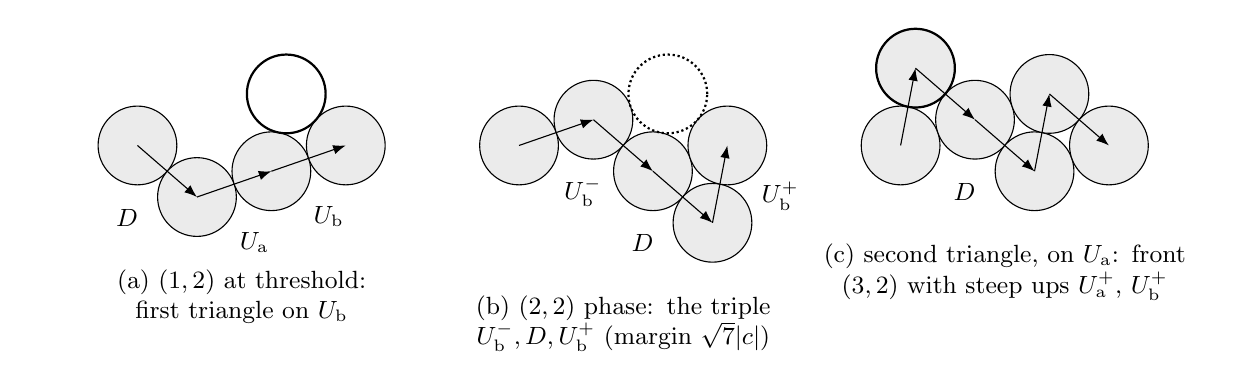
\begin{tikzpicture}[x=1.0cm,y=1.0cm]
% generated by verify/schematic_figures.py
\begin{scope}[shift={(0.000,0)}]
\draw[fill=black!8] (0.0000,0.0000) circle (0.5);
\draw[fill=black!8] (0.7559,-0.6547) circle (0.5);
\draw[fill=black!8] (1.7008,-0.3273) circle (0.5);
\draw[fill=black!8] (2.6458,0.0000) circle (0.5);
\draw[thick] (1.8898,0.6547) circle (0.5);
\draw[-{Latex[length=1.6mm]}] (0.0000,0.0000)--(0.7559,-0.6547);
\node[font=\small] at (-0.1327,-0.9170) {$D$};
\draw[-{Latex[length=1.6mm]}] (0.7559,-0.6547)--(1.7008,-0.3273);
\node[font=\small] at (1.4837,-1.2280) {$U_{\mathrm a}$};
\draw[-{Latex[length=1.6mm]}] (1.7008,-0.3273)--(2.6458,0.0000);
\node[font=\small] at (2.4286,-0.9007) {$U_{\mathrm b}$};

\node[font=\small,align=center,text width=5.2cm,anchor=north] at (1.3229,-1.4547) {(a) $(1,2)$ at threshold:\\first triangle on $U_{\mathrm b}$};
\end{scope}
\begin{scope}[shift={(4.846,0)}]
\draw[fill=black!8] (0.0000,0.0000) circle (0.5);
\draw[fill=black!8] (0.9449,0.3273) circle (0.5);
\draw[fill=black!8] (1.7008,-0.3273) circle (0.5);
\draw[fill=black!8] (2.4568,-0.9820) circle (0.5);
\draw[fill=black!8] (2.6458,0.0000) circle (0.5);
\draw[densely dotted,thick] (1.8898,0.6547) circle (0.5);
\draw[-{Latex[length=1.6mm]}] (0.0000,0.0000)--(0.9449,0.3273);
\draw[-{Latex[length=1.6mm]}] (0.9449,0.3273)--(1.7008,-0.3273);
\node[font=\small] at (0.8122,-0.5896) {$U_{\mathrm b}^-$};
\draw[-{Latex[length=1.6mm]}] (1.7008,-0.3273)--(2.4568,-0.9820);
\node[font=\small] at (1.5682,-1.2443) {$D$};
\draw[-{Latex[length=1.6mm]}] (2.4568,-0.9820)--(2.6458,0.0000);
\node[font=\small] at (3.3172,-0.6384) {$U_{\mathrm b}^+$};

\node[font=\small,align=center,text width=5.2cm,anchor=north] at (1.3229,-1.7820) {(b) $(2,2)$ phase: the triple\\$U_{\mathrm b}^-,D,U_{\mathrm b}^+$ (margin $\sqrt7|c|$)};
\end{scope}
\begin{scope}[shift={(9.692,0)}]
\draw[fill=black!8] (0.0000,0.0000) circle (0.5);
\draw[fill=black!8] (0.1890,0.9820) circle (0.5);
\draw[fill=black!8] (0.9449,0.3273) circle (0.5);
\draw[fill=black!8] (1.7008,-0.3273) circle (0.5);
\draw[fill=black!8] (1.8898,0.6547) circle (0.5);
\draw[fill=black!8] (2.6458,0.0000) circle (0.5);
\draw[thick] (0.1890,0.9820) circle (0.5);
\draw[-{Latex[length=1.6mm]}] (0.0000,0.0000)--(0.1890,0.9820);
\draw[-{Latex[length=1.6mm]}] (0.1890,0.9820)--(0.9449,0.3273);
\draw[-{Latex[length=1.6mm]}] (0.9449,0.3273)--(1.7008,-0.3273);
\node[font=\small] at (0.8122,-0.5896) {$D$};
\draw[-{Latex[length=1.6mm]}] (1.7008,-0.3273)--(1.8898,0.6547);
\draw[-{Latex[length=1.6mm]}] (1.8898,0.6547)--(2.6458,0.0000);

\node[font=\small,align=center,text width=5.2cm,anchor=north] at (1.3229,-1.1273) {(c) second triangle, on $U_{\mathrm a}$: front $(3,2)$ with steep ups $U_{\mathrm a}^+$, $U_{\mathrm b}^+$};
\end{scope}

\end{tikzpicture}
\caption{The first Fibonacci transition at the $(1,2)$ threshold tiling (exact coordinates; open disks are
new triangle disks). In (b) the dotted disk marks where a pentagon would sit: at the limit it touches three
disks, and with shrinking disks it misses by $\sqrt7|c|$ to first order.}\label{fig:stepone}
\end{figure}

\subsection{The \texorpdfstring{$(1,2)$}{(1,2)} phase} A front with one down vector has a single notch, $D$ followed by an
up vector, so in a rhombic phase the two up vectors pass $D$ alternately. Each pass turns $D$ by
$-c\cos\beta_U>0$ and the passing up vector by $c\cos\beta_D<0$ (Corollary~\ref{cor:rates}), so
the notch hinge $\pi-(\beta_U-\beta_D)$ increases steadily, while by
Proposition~\ref{prop:frozen} the ratio $\Ua/\Ub$ stays $e^{i\eps}$ up to $O(|c|)$. Along the
way the configuration follows the $(1,2)$ lattice fronts from $F(\beta,\eps)$ to the threshold of
Lemma~\ref{lem:threshold}, up to $O(|\eps|+|c|)$. On that compact path the notch hinge stays in
$(60^\circ,120^\circ)$ and the $1,2$-notch has $\gamma+\tau>4\pi/3$ by a margin bounded below, so
by~\cite[Prop.~4.3]{GD} and Lemma~\ref{lem:apex} the only valid offspring is the rhombus.

The phase ends at the first step at which a triangle candidate is valid. At the threshold tiling this is
a triple site: the triangle on $D$, the triangle on the up vector that follows it, and the rhombus over the
notch disk are one and the same disk, touching three disks. So the switch does not happen at a hinge of
exactly $120^\circ$ once $c\ne0$ (it happens at $120^\circ+O(|c|)$), and which triangle is placed is decided
at first order, not by an order-one margin. Lemma~\ref{lem:shared} settles it: whenever the triangle on
$D$ is valid, the triangle on the up vector is valid and no higher, with equality only when the two are
the same disk, which is then inserted on the up vector. So the first triangle rests on an up vector. Call
it $\Ub$ and the other $\Ua$. (When $|c|\ll|\eps|$, $\Ub$ is the less steep one; Theorem~\ref{thm:A} does not
need that.)

\subsection{Two candidates sharing a contact}
Every near-tie in this section has the same shape. Put
$u_*=\beta_{\min}=\arctan(\sqrt3/5)$ and let
\[
U=e^{iu_*},\qquad S=e^{i(u_*-\pi/3)},\qquad V=e^{i(u_*+\pi/3)}
\]
be the unit up, down and steep up vectors of the $(1,2)$ threshold tiling (Lemma~\ref{lem:threshold}).

\begin{lemma}[Shared contact]\label{lem:shared}
Let $A$, $B$, $E$ be disks of a front and $Q_*$ a point at which, at $\eps=c=0$, a unit disk touches all
three, with contact normals
\[
Q_*-A=U,\qquad Q_*-B=V,\qquad Q_*-E=-S.
\]
For configurations in a small enough neighbourhood of this one (positions, diameters, and $|c|$ small),
let $T$ be the placement touching $A$ and $B$ and $R$ the placement touching $B$ and $E$, on the branches
through $Q_*$. If $T$ clears $E$, then $R$ clears $A$ and $\Imag R\le\Imag T$, with equality only if $T=R$.
Every other disk of the stack, older disks included, clears both.
\end{lemma}

\begin{proof}
For a disk $P$ write $f_P(X)=|X-P|-\tfrac12\bigl(d_P+d(X)\bigr)$, with $d(X)=b_0+c\Imag X$; $X$ clears $P$
when $f_P(X)\ge0$. Near $Q_*$ the curve $f_B=0$ is a graph $y=h(x)$, since its $y$-derivative is close to
$\Imag V>0$, and $h'=-\Real V/(\Imag V-c/2)+o(1)<0$ because both coordinates of $V$ are positive. Along it
put $g_A(x)=f_A(x,h(x))$ and $g_E(x)=f_E(x,h(x))$. At the limit
\[
g_A'=\frac{\sin(\pi/3)}{\sin(u_*+\pi/3)}>0,\qquad g_E'=\frac{\sin(-\pi/3)}{\sin(u_*+\pi/3)}<0,
\]
and both signs persist nearby. $T$ is the zero $x_T$ of $g_A$ and $R$ the zero $x_R$ of $g_E$, unique by the
implicit function theorem since the contact normals are not parallel. If $T$ clears $E$ then
$g_E(x_T)\ge0=g_E(x_R)$, so $x_T\le x_R$ and $\Imag T=h(x_T)\ge h(x_R)=\Imag R$; and
$g_A(x_R)\ge g_A(x_T)=0$, so $R$ clears $A$. Equality forces $x_T=x_R$.

For the other disks: before the first offending event every step is a triangle (which removes nothing) or
a rhombus (which removes a notch bottom lower than its parents), so no centre in the stack is higher than
the highest front disk, whose height tends to that of $B$, below $Q_*$. The directions from $Q_*$ to $A$, $B$,
$E$ are $u_*+180^\circ$, $u_*+240^\circ$, $u_*+300^\circ$, about $199^\circ$, $259^\circ$, $319^\circ$, and every
direction in the lower half-plane is within less than $60^\circ$ of one of them. A unit disk centred at
$Q_*+rn$, $0<r\le1$, $n$ in the lower half-plane, would therefore lie at distance
$\sqrt{1+r^2-2r\cos\theta}<1$ from that parent, $\theta<60^\circ$, overlapping it. So at the limit no
other disk meets $Q_*$; any disk overlapping a nearby candidate $X$ has its centre within
$d(X)/(1-|c|/2)$ of $X$, so by compactness the exclusion persists in a neighbourhood.
\end{proof}

\noindent In words: both candidates touch $B$, and the curve of such positions descends to the right. Clearing
the right-hand disk $E$ forces $T$ onto the higher part of that curve. The lemma is used twice. In a down-up
notch $A\xrightarrow{S}B\xrightarrow{U}E$ ($E=B+U$), $T$ is the triangle on the down vector and $R$ the
triangle on the up vector. In the words $\Ua\,\dn{\Ub}\,D\,\up{\Ub}$ and $\Ua\,D\,\dn{\Ub}\,\up{\Ub}$ below,
$A,B$ are the ends of the first down vector and $E$ the end of the up vector $\up{\Ub}$, so $T$ is a triangle
on a down vector and $R$ the rhombus. The comparison is exact; it does not need a margin.

\subsection{The \texorpdfstring{$(2,2)$}{(2,2)} phase} After the first triangle the front is $\Ua,D,\up{\Ub},\dn{\Ub}$,
where $\up{\Ub}$ and $\dn{\Ub}$ are the new up and down vectors. At $\eps=c=0$ these are the four vectors of
the $(1,2)$ threshold tiling: $\Ua$ at $\beta_{\min}$, $D$ and $\dn{\Ub}$ both at $\beta_{\min}-60^\circ$, and
$\up{\Ub}$ at $\beta_{\min}+60^\circ$. The phase runs through four words, read cyclically from $\Ua$:
\[
\Ua\,D\,\up{\Ub}\,\dn{\Ub}\;\to\;\Ua\,\dn{\Ub}\,D\,\up{\Ub}\;\to\;\Ua\,\dn{\Ub}\,\up{\Ub}\,D
\;\to\;\Ua\,D\,\dn{\Ub}\,\up{\Ub}\;\to\;\cdots,
\]
in which $\Ua$ and $\up{\Ub}$ pass strictly alternately.

\begin{lemma}\label{lem:alternation}
In each of the four words at the limit tiling, the lowest valid position is unique up to the
degenerate coincidences listed below, and every valid position at another location is at least
$\sqrt{3/28}\,b_0\approx0.327\,b_0$ higher. Consequently the passes alternate for $|\eps|,|c|$ small, and
the gap between $\Ua$ and $\up{\Ub}$ is $1+P_{\Ua}-P_{\up{\Ub}}\in\{1,2\}$; it is never empty.
\end{lemma}

\begin{proof}
Each of the four words is a word in the vectors of the $(1,2)$ threshold tiling, so in the rational
model with $7$ in place of $19$ every candidate position is a rational point: pairs at distance $1$, $\sqrt3$
and $2$ have their apexes at lattice points and farther pairs have none. The candidates were enumerated and
compared in exact rational arithmetic (\texttt{verify/exact\_limits.py}; an independent interval-arithmetic
check is \texttt{verify/certify\_limits.py}). The coincidences are exact identities of rational points, of two
kinds: in the first and third words a triangle on a down vector, the triangle on $\Ua$ and a rhombus; in the
second and fourth a triangle on a down vector, a rhombus and a pentagon. Both are treated below. The value $\sqrt{3/28}$ is exact: in the word $\Ua\,D\,\up{\Ub}\,\dn{\Ub}$
the lowest position is the apex $w_3+\Ua$ of the triangle on $(\dn{\Ub},\Ua)$ and the next is the
rhombus apex $w_1+\up{\Ub}$, half a unit of $Y$ higher in the rational model. The gap formula is~\eqref{eq:gaps} applied
to alternating passes.
\end{proof}

\subsection{No pentagon in the first transition} A pentagon needs a three-vector notch whose two hinges
sum to at most $240^\circ$. Three such triples are degenerate at zeroth order in the $(2,2)$ phase.

The triple $D,\Ua,\up{\Ub}$ (one down, two ups) needs $\Ua$ immediately followed by $\up{\Ub}$, an empty gap,
which Lemma~\ref{lem:alternation} excludes.

The other two have two downs and one up, namely $\dn{\Ub},D,\up{\Ub}$ in the word
$\Ua\,\dn{\Ub}\,D\,\up{\Ub}$ and $D,\dn{\Ub},\up{\Ub}$ in the word $\Ua\,D\,\dn{\Ub}\,\up{\Ub}$. By~\eqref{eq:hinge} the hinge sum minus
$240^\circ$ telescopes to
\[
m_j=\tfrac{2\pi}3-\bigl(\arg\up{\Ub}-\arg d_j\bigr),
\]
where $d_j$ is the first down vector of the triple ($\dn{\Ub}$, respectively $D$); the middle vector drops out.
Write $u$ for the bearing of $\Ub$ when it is split, $a$ for that of $\Ua$ and $d$ for that of $D$, all within
$\delta$ of their threshold values, and use the two first-order rules: a triangle on $\Ub$ creates
$\arg\up{\Ub}=u+\tfrac\pi3+\tfrac c2\cos(u-\tfrac\pi3)$ and $\arg\dn{\Ub}=u-\tfrac\pi3-\tfrac c2\cos(u+\tfrac\pi3)$
(Lemma~\ref{lem:triangle}), and a pass of an up bearing $a$ over a down bearing $d$ sends
$a\mapsto a+c\cos d$, $d\mapsto d-c\cos a$ (Corollary~\ref{cor:rates}), each up to $O(c^2)$.

For $d_j=\dn{\Ub}$: the triple first forms after $\Ua$ passes $\dn{\Ub}$, so
\begin{equation}\label{eq:ddu}
m_{\dn{\Ub}}=-c\bigl(\tfrac12\cos u+\cos a\bigr)+O(\delta|c|+c^2)=\tfrac{15}{4\sqrt7}|c|+O(\delta|c|+c^2)\approx1.417\,|c|,
\end{equation}
with $\cos\beta_{\min}=5/(2\sqrt7)$. For $d_j=D$: put $\eta_0=\tfrac\pi3-(u-d)$ when the first triangle is
placed. That triangle clears its left neighbour, and the clearance is
$\tfrac{\sqrt3}2\eta_0-\tfrac34c\sin(u_*+\tfrac\pi3)+O(\eta_0^2+\delta|c|+c^2)$ with root exactly $\eta_0=0$ at
$c=0$, so $\eta_0\ge\tfrac{9}{4\sqrt7}c+O(\delta|c|+c^2)$. Before the triple forms, $\up{\Ub}$ and then $\Ua$
have passed $D$, so
\begin{equation}\label{eq:dud}
m_D=\eta_0-c\bigl(\tfrac12\cos s_*+\cos s_*+\cos v_*+\cos u_*\bigr)+O(\delta|c|+c^2)
\ge\tfrac{15}{4\sqrt7}|c|+O(\delta|c|+c^2),
\end{equation}
since the cosine sum is $6/\sqrt7$ (here $s_*=u_*-\tfrac\pi3$, $v_*=u_*+\tfrac\pi3$).

Later passes only increase either margin: every rhombus that changes $m_j$ decreases $\arg\up{\Ub}$ or
increases $\arg d_j$, by $|c|$ times a cosine bounded away from zero, up to $O(c^2)$. So no unsigned error
accumulates over the phase, however long it is, and both margins stay at least $\tfrac{15}{4\sqrt7}|c|$ up to
$O(\delta|c|+c^2)$. A pentagon needs more than a negative margin: reflecting centres by $z\mapsto-\bar z$ and
reversing the front order (so front vectors become $v\mapsto\bar v$) turns either triple into a
one-down-two-up notch whose down vector has $\cos=1/(2\sqrt7)$, $\sin=-3\sqrt3/(2\sqrt7)$, and
Lemma~\ref{lem:pent} below then requires the margin to be below $-\kappa_2|c|$ with
$\kappa_2=13/(4\sqrt7)\approx1.228$. The two requirements are separated by
\[
\tfrac{15}{4\sqrt7}+\tfrac{13}{4\sqrt7}=\sqrt7\approx2.646
\]
times $|c|$, so no pentagon forms.

\subsection{No triangle on a down vector} In the words $\Ua\,\dn{\Ub}\,D\,\up{\Ub}$ and $\Ua\,D\,\dn{\Ub}\,\up{\Ub}$
the exact tables put a triangle on the first down vector, the rhombus on the next two vectors and the
pentagon of the triple above at one point (\texttt{verify/exact\_limits.py}). The pentagon is excluded, and
by Lemma~\ref{lem:shared} the rhombus is valid and no higher whenever the triangle is valid. In fact the
gap is strict along the trajectory: expanding both placements to first order gives, with $b$ the diameter
of the first disk of the triple,
\[
\begin{aligned}
\frac{\Imag T-\Imag R}{b}&=m_j\Bigl(\frac1{2\sqrt7}+O(\delta)\Bigr)-c\Bigl(\frac{13}{56}+O(\delta)\Bigr)+O(c^2)\\
&\ge|c|\Bigl(\frac{15}{56}+\frac{13}{56}\Bigr)-O(\delta|c|+c^2)=\frac{|c|}2-O(\delta|c|+c^2),
\end{aligned}
\]
using~\eqref{eq:ddu} and~\eqref{eq:dud}. In simulations the smallest observed value of
$(\Imag T-\Imag R)/(b|c|)$ is $0.4997$ (\texttt{verify/down\_triangle\_exclusion.py}).

\begin{proof}[Proof of Theorem~\ref{thm:A}]
In the $(1,2)$ phase the only offspring is the rhombus until a triangle first becomes valid, at a triple
site where Lemma~\ref{lem:shared} places it on an up vector. In the $(2,2)$ phase the passes alternate with
the margin of Lemma~\ref{lem:alternation}, and the coincidences at the lowest location are of two kinds. In
the words $\Ua\,D\,\up{\Ub}\,\dn{\Ub}$ and $\Ua\,\dn{\Ub}\,\up{\Ub}\,D$ a triangle on the down vector before $\Ua$
meets the triangle on $\Ua$ and a rhombus, at the down-up notch before $\Ua$. By Lemma~\ref{lem:shared} for
that notch no triangle on the down vector is placed; the triangle on $\Ua$, when valid, is the intended
second triangle, and at an exact tie the same disk is inserted on $\Ua$. In the other two words a triangle
on a down vector meets the rhombus and a pentagon; the pentagon is excluded and the rhombus is placed, as
shown above. The remaining comparisons hold at the limit tilings with margins of order one, and the
configurations stay within $O(|\eps|+|c|)$ of the limit, because the $(2,2)$ phase lasts $O(|\eps|/|c|+1)$
steps with drift $O(|c|)$ per step; by Lemma~\ref{lem:uniform} those margins persist for $|\eps|<\eps_0$ and
$|c|<c_0$. The margins of order $|c|$, \eqref{eq:ddu} and~\eqref{eq:dud}, are signed and only increase during
the phase. The front after the second triangle has up vectors $\up{\Ua},\up{\Ub}$ and down vectors
$D,\dn{\Ua},\dn{\Ub}$.
\end{proof}

\section{The second transition}\label{sec:steptwo}

This section collects the evidence for the delayed mechanism. Its target is the following statement,
which we do not prove.

\begin{conjecture}[Delayed pentagon]\label{thm:B}
For every $\beta\in(\beta_{\min},\pi/6)$ there are $\eps_0>0$ and $K\ge1$ such that for
$0<|\eps|<\eps_0$ and $0<|c|<|\eps|/K$, stacking from $F(\beta,\eps)$ performs a pentagon transition
after its front first has parastichy numbers $(3,2)$ and before it first has $(8,5)$, at most five
transitions after the first triangle threshold of the $(3,2)$ phase.
\end{conjecture}

\noindent In four of the six first-order event calculations, and in the recorded simulations, the
pentagon comes before $(3,5)$, so it interrupts the second Fibonacci transition. In the remaining two
cases a tie that first-order analysis does not break decides whether it comes just before or just
after the third triangle of step two; both branches are followed (Section~\ref{sec:burst}). The
calculation is not a certificate for the nonlinear dynamics: a candidate whose clearance vanishes at
both retained orders can disappear at higher order, exposing a different lowest valid candidate.
Section~\ref{sec:burst} ends with the remaining verification problem.

\subsection{What the first transition leaves behind}
Up/up and down/down ratios are frozen through every rhombic phase (Proposition~\ref{prop:frozen}), and each
triangle multiplies its vector by $\omega$ or $\bar\omega$ up to $O(c)$, with corrections that agree to
zeroth order for $\Ua$ and $\Ub$ (Lemma~\ref{lem:triangle}). Hence, at the end of the first transition,
\begin{equation}\label{eq:inherit}
\frac{\up{\Ua}}{\up{\Ub}}=e^{i\eps}\bigl(1+O(c)\bigr),\qquad
\frac{\dn{\Ua}}{\dn{\Ub}}=e^{i\eps}\bigl(1+O(c)\bigr),\qquad
\frac{D}{\dn{\Ub}}=1+O(c),
\end{equation}
and by Proposition~\ref{prop:frozen} again these ratios hold through the whole $(3,2)$ phase. In words:
the two new up vectors still differ in angle by $\eps$, and so do the two down vectors born from $\Ua$
and $\Ub$, while $D$ and $\dn{\Ub}$ are parallel up to $O(c)$. In the sampled
simulations, the up mismatch at the start of step two is well fitted by
$\theta=|\eps|-\kappa_1|c|$ with slope close to one
and $\kappa_1$ between $1.399$ and $1.666$ for $\beta\in[0.42,0.523]$ (Table~\ref{tab:kappa1}); $\kappa_1$
collects the $O(c)$ terms of~\eqref{eq:inherit}, and we have no closed form for it.

\begin{lemma}[The $(3,2)$ phase]\label{lem:32phase}
Suppose no pentagon occurs during the $(3,2)$ phase. Then every step of the phase is the rhombus at the
lowest lattice position, until a triangle candidate first becomes valid, at a notch hinge of
$120^\circ+O(|c|)$; the front then lies within
$O(|c|)$ of the front $K_\eps(w)$ determined by~\eqref{eq:inherit}, by one of the six cyclic words $w$ of the
phase, by closure and by the threshold condition.
\end{lemma}

\begin{proof}
By~\eqref{eq:inherit} the front is within $O(|\eps|+|c|)$ of a $(3,2)$ rhombic lattice front with down
vector $D$ and up vector $U$. Closure gives $3\Imag D+2\Imag U=0$, so lattice points $aU+bD$ have heights
$\tfrac12|\Imag D|(3a-2b)$: distinct positions modulo the period are separated by at least
$\tfrac12|\Imag D|\ge\tfrac12 b\sin23.4^\circ>0.19\,b$ along the whole phase, since $|\beta_D|$ decreases from about
$41^\circ$ to $23.4^\circ$. Rhombus candidates are lattice positions, so the order of the passes is the
lattice order with that margin. Triangle candidates overlap a neighbour while every hinge is below
$120^\circ-K|c|$ for a constant $K$ (the exact switching boundary moves with $c$, as in
Section~\ref{sec:stepone}). By assumption no pentagon is placed. The front thus follows the six-word cycle of the
lattice, and at the first threshold crossing it is determined, up to $O(c)$, by the frozen
ratios~\eqref{eq:inherit}, the word, closure and the hinge $120^\circ$, up to $O(c)$.
\end{proof}

The hypothesis isolates the unresolved case of Conjecture~\ref{thm:B}: a pentagon in the
$(3,2)$ phase would already give its asserted breakdown. In the six words the two up vectors are never adjacent, so no one-down-two-up
notch exists during the phase.

\subsection{When a pentagon fits}
\begin{figure}[t]
\centering
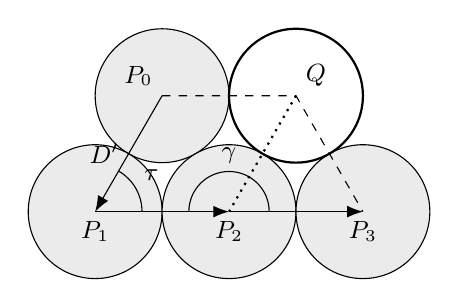
\begin{tikzpicture}[scale=1.7,every node/.style={font=\small}]
\coordinate (P0) at (0.5,0.8660); \coordinate (P1) at (0,0); \coordinate (P2) at (1,0); \coordinate (P3) at (2,0);
\coordinate (Q) at (1.5,0.8660);
\foreach \p in {P0,P1,P2,P3} \draw[fill=black!8] (\p) circle (0.5);
\draw[thick,fill=white,fill opacity=0.7] (Q) circle (0.5);
\foreach \p/\l/\a in {P0/P_0/above left,P1/P_1/below,P2/P_2/below,P3/P_3/below,Q/Q/above right} \node[\a] at (\p) {$\l$};
\draw[-{Latex[length=2mm]}] (P0)--(P1) node[midway,left] {$D'$};
\draw[-{Latex[length=2mm]}] (P1)--(P2);
\draw[-{Latex[length=2mm]}] (P2)--(P3);
\draw[dashed] (P0)--(Q)--(P3);
\draw[dotted,thick] (Q)--(P2);
\draw (0.35,0) arc (0:60:0.35); \node at (0.42,0.27) {$\tau$};
\draw (1.3,0) arc (0:180:0.3); \node at (1.0,0.42) {$\gamma$};
\end{tikzpicture}
\caption{The degenerate pentagon. With hinges $\tau=60^\circ$ and $\gamma=180^\circ$ the disk $Q$
touching $P_0$ and $P_3$ also touches $P_2$ (dotted), and $|Q-P_1|=\sqrt3$. Turning $U_2$ up by $\theta$
lifts $Q$ off $P_2$; shrinking disks press it back by $\kappa_2|c|$.}\label{fig:pent}
\end{figure}

Take a notch $P_0\xrightarrow{D'}P_1\xrightarrow{U_1}P_2\xrightarrow{U_2}P_3$ with hinges
$\tau=h(D',U_1)=60^\circ+\sigma$ (the cushion $\sigma$) and $\gamma=h(U_1,U_2)=180^\circ-\theta$ (the up mismatch
$\theta$). At constant diameter a pentagon fits exactly when $\gamma+\tau\le240^\circ$~\cite[Prop.~4.3]{GD},
that is, when $\theta\ge\sigma$. The next lemma gives the first correction for shrinking disks.

\begin{lemma}[Pentagon with shrinking disks]\label{lem:pent}
Let $\beta_D$ be the bearing of $D'$. Near the degenerate point of Figure~\ref{fig:pent}, the disk $Q$
touching $P_0$ and $P_3$ clears $P_2$ if and only if
\[
\theta\ge\sigma+\kappa_2(\beta_D)\,|c|+O\bigl(|c|(|\theta|+|\sigma|+|c|)\bigr),\qquad
\kappa_2(\beta_D)=-\tfrac14\bigl(\cos\beta_D+3\sqrt3\sin\beta_D\bigr),
\]
and $|Q-P_1|=\sqrt3\,b_0$ at the degenerate reference configuration. Thus $P_1$
remains strictly clear in a sufficiently small neighbourhood.
\end{lemma}

\begin{proof}
Work in the frame where $U_1$ points along the real axis, with unit diameter at $P_1=0$; heights are
$\eta(x,y)=sx+ky$ with $s=\sin\alpha$, $k=\cos\alpha$, $\alpha=\arg U_1$ in the cylinder frame, and put
$t=\sin(\alpha+\pi/3)=\tfrac s2+\tfrac{\sqrt3}2k$. At the degenerate point $P_0=\omega$, $P_2=1$, $P_3=2$,
$Q=\tfrac32+\tfrac{\sqrt3}2 i$. Let $G=|Q-P_2|^2-\bigl(\tfrac{d_2+d_Q}{2}\bigr)^2$; $Q$ clears $P_2$ when $G\ge0$.

\emph{Along the mismatch} ($c=0$): $P_3$ moves with velocity $i$ and $Q$ keeps touching $P_0$ and $P_3$.
By~\eqref{eq:tangency} with zero right-hand sides, $Q'=(0,1)$, so $\partial_\theta G=2(Q-P_2)\cdot Q'=\sqrt3$.

\emph{Along the rate} ($\theta=\sigma=0$): the side lengths are mean diameters, which gives the velocities
$P_2'=(\tfrac s2,0)$, $P_3'=(2s,0)$, $P_0'=\tfrac t2\,\omega$ (hinges held fixed). The tangencies with $P_0$
and $P_3$ give $Q'_x=\tfrac s2+\tfrac54t$ and $\sqrt3\,Q'_y=\tfrac{6s+9t}4$, and then
$\partial_cG=2(Q-P_2)\cdot(Q'-P_2')-(\eta(P_2)+\eta(Q))=\tfrac{5t-s}2$.

At $c=0$ the boundary is exactly $\theta=\sigma$~\cite[Prop.~4.3]{GD}, so $G(\theta,\sigma,0)$ vanishes on
$\theta=\sigma$ and, $G$ being analytic, $G(\theta,\sigma,0)=(\theta-\sigma)\bigl(\sqrt3+O(|\theta|+|\sigma|)\bigr)$. Adding
the rate, $G=(\theta-\sigma)\bigl(\sqrt3+O(|\theta|+|\sigma|)\bigr)+c\bigl(\tfrac{5t-s}2+O(|\theta|+|\sigma|+|c|)\bigr)$, so
the boundary $G=0$ is $\theta=\sigma-\frac{5t-s}{2\sqrt3}\,c+O\bigl(|c|(|\theta|+|\sigma|+|c|)\bigr)$. With $\alpha=\beta_D+2\pi/3$ one has
$t=-\sin\beta_D$ and $\frac{5t-s}{2\sqrt3}=\kappa_2(\beta_D)$. Finally $|Q-P_1|^2=\tfrac94+\tfrac34=3$.
\end{proof}

A least-squares fit of the exact boundary over $\beta_D\in[-105^\circ,-60^\circ]$ returns the coefficients
$-0.25000$ and $-1.29904$ of $\cos\beta_D$ and $\sin\beta_D$ (\texttt{verify/local\_existence\_fit.out}). At the steep child of the tiling $K_0$ below,
$\cos\beta_D=1/(2\sqrt{19})$, $\sin\beta_D=-5\sqrt3/(2\sqrt{19})$ and $\kappa_2=11/(2\sqrt{19})\approx1.262$.

\subsection{The tiling \texorpdfstring{$K_0$}{K0} and the placement margins}
\begin{figure}[t]
\centering
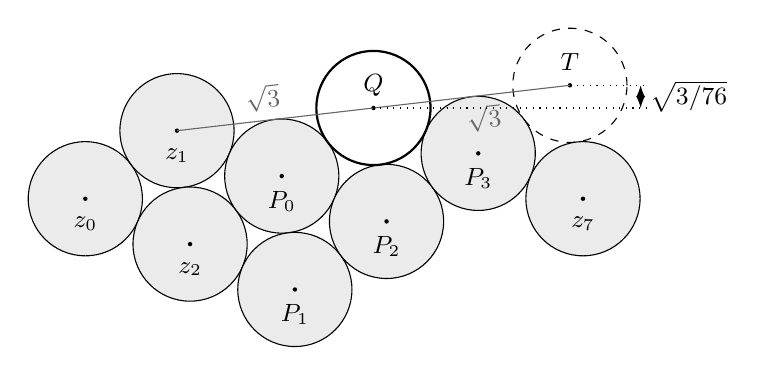
\begin{tikzpicture}[x=1.45cm,y=1.45cm,every node/.style={font=\small}]
\def\sx{0.229416}\def\sy{0.397360}
\foreach \X/\Y/\n in {0/0/z_0,3.5/1.5/z_1,4/-1/z_2,7.5/0.5/P_0,8/-2/P_1,11.5/-0.5/P_2,15/1/P_3,19/0/z_7}
  {\draw[fill=black!8] (\X*\sx,\Y*\sy) circle (0.5); \node at (\X*\sx,\Y*\sy-0.22) {$\n$}; \fill (\X*\sx,\Y*\sy) circle (0.8pt);}
\draw[thick] (11*\sx,2*\sy) circle (0.5); \fill (11*\sx,2*\sy) circle (0.8pt); \node at (11*\sx,2*\sy+0.2) {$Q$};
\draw[dashed] (18.5*\sx,2.5*\sy) circle (0.5); \fill (18.5*\sx,2.5*\sy) circle (0.8pt); \node at (18.5*\sx,2.5*\sy+0.2) {$T$};
\draw[black!60] (3.5*\sx,1.5*\sy)--node[pos=0.45,above,sloped] {$\sqrt3$} (11*\sx,2*\sy);
\draw[black!60] (11*\sx,2*\sy)--node[pos=0.55,below,sloped] {$\sqrt3$} (18.5*\sx,2.5*\sy);
\draw[dotted] (11*\sx,2*\sy)--(21.5*\sx,2*\sy); \draw[dotted] (18.5*\sx,2.5*\sy)--(21.5*\sx,2.5*\sy);
\draw[{Latex[length=1.5mm]}-{Latex[length=1.5mm]}] (21.2*\sx,2*\sy)--(21.2*\sx,2.5*\sy) node[midway,right] {$\sqrt{3/76}$};
\end{tikzpicture}
\caption{The tiling $K_0$ at the moment the pentagon is placed (unit diameters). The pentagon disk $Q$
touches $P_0$, $P_2$ and $P_3$. The lagging triangle $T$ on the last down vector is $\sqrt{3/76}$ higher,
and the burst disk $z_1$ is at distance $\sqrt3$ and $\sqrt{3/76}$ lower.}\label{fig:K0}
\end{figure}

As $\eps,c\to0$ the burst of step two converges to the $(3,2)$ threshold lattice with two triangles fired.
The front at the moment of the pentagon is the word $U\,S\,U\,S\,U\,U\,D$ in the vectors~\eqref{eq:K0vectors},
period $\sqrt{19}$, with points $z_0,\dots,z_7$ and $P_0,\dots,P_3=z_3,\dots,z_6$ (Figure~\ref{fig:K0}). In the
rational model $Q=(11,2)$, $T=z_6+U=(18.5,2.5)$ and $z_1=(3.5,1.5)$.

\begin{lemma}\label{lem:K0}
In $K_0$, $Q$ touches $P_0$, $P_2$ and $P_3$ and is at distance $\sqrt3$ from $P_1$; $T$ touches $z_6$ and $z_7$;
$|T-Q|=|Q-z_1|=\sqrt3$; and $\Imag(T-Q)=\Imag(Q-z_1)=\sqrt{3/76}\approx0.1987$. Every other valid position is
at least $2\sqrt{3/76}$ above $Q$.
\end{lemma}

\begin{proof}
The first four statements are the rational identities $\Delta X^2+3\Delta Y^2\in\{19,57\}$ and $\Delta Y=\tfrac12$.
The last is an enumeration in exact rational arithmetic in the same model (\texttt{exact\_limits.py}): the
pentagon, rhombus and triangle at $Q$ are the same rational point, the three positions at $T$ likewise, and
every other location has $\Delta Y\ge1$, that is, lies at least $2\sqrt{3/76}$ above $Q$.
\end{proof}

\subsection{The burst}\label{sec:burst}
It remains to follow the few events between the first threshold crossing of the $(3,2)$ phase and the
pentagon. Figure~\ref{fig:burst} shows one of the six cases at the limit $\eps=c=0$.

\begin{figure}[t]
\centering
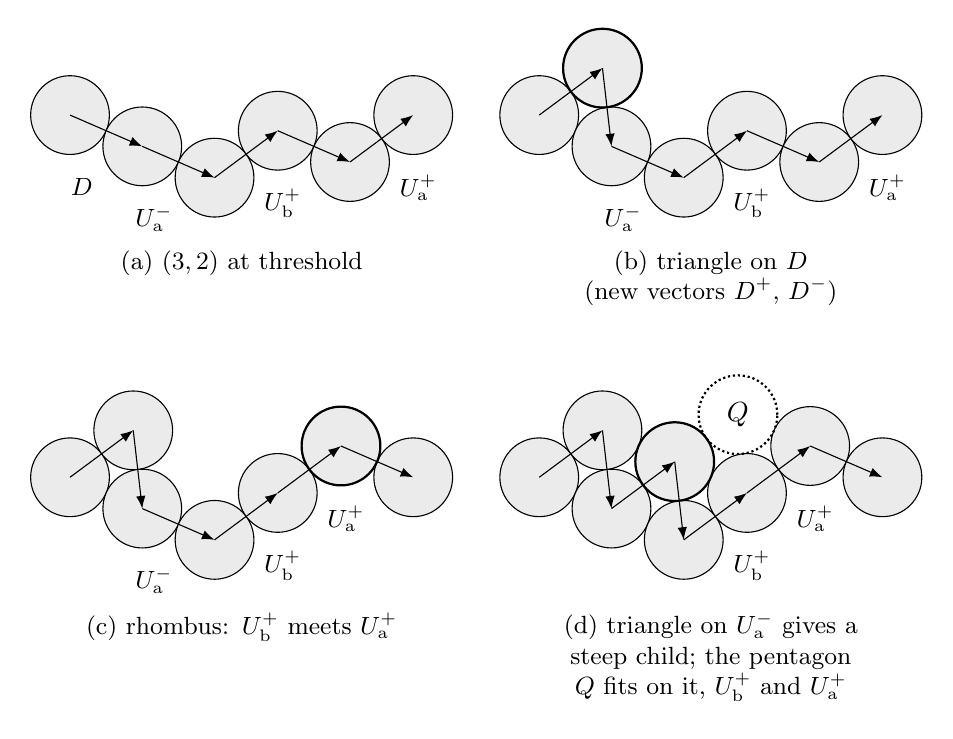
\begin{tikzpicture}[x=1.0cm,y=1.0cm]
% generated by verify/schematic_figures.py
\begin{scope}[shift={(0.000,0.000)}]
\begin{scope}[shift={(0.000,0)}]
\draw[fill=black!8] (0.0000,0.0000) circle (0.5);
\draw[fill=black!8] (0.9177,-0.3974) circle (0.5);
\draw[fill=black!8] (1.8353,-0.7947) circle (0.5);
\draw[fill=black!8] (2.6383,-0.1987) circle (0.5);
\draw[fill=black!8] (3.5559,-0.5960) circle (0.5);
\draw[fill=black!8] (4.3589,0.0000) circle (0.5);
\draw[-{Latex[length=1.6mm]}] (0.0000,0.0000)--(0.9177,-0.3974);
\node[font=\small] at (0.1489,-0.9145) {$D$};
\draw[-{Latex[length=1.6mm]}] (0.9177,-0.3974)--(1.8353,-0.7947);
\node[font=\small] at (1.0666,-1.3118) {$U_{\mathrm a}^-$};
\draw[-{Latex[length=1.6mm]}] (1.8353,-0.7947)--(2.6383,-0.1987);
\node[font=\small] at (2.7017,-1.1230) {$U_{\mathrm b}^+$};
\draw[-{Latex[length=1.6mm]}] (2.6383,-0.1987)--(3.5559,-0.5960);
\draw[-{Latex[length=1.6mm]}] (3.5559,-0.5960)--(4.3589,0.0000);
\node[font=\small] at (4.4223,-0.9243) {$U_{\mathrm a}^+$};

\node[font=\small,align=center,text width=5.2cm,anchor=north] at (2.1794,-1.5947) {(a) $(3,2)$ at threshold};
\end{scope}
\end{scope}
\begin{scope}[shift={(5.959,0.000)}]
\begin{scope}[shift={(0.000,0)}]
\draw[fill=black!8] (0.0000,0.0000) circle (0.5);
\draw[fill=black!8] (0.8030,0.5960) circle (0.5);
\draw[fill=black!8] (0.9177,-0.3974) circle (0.5);
\draw[fill=black!8] (1.8353,-0.7947) circle (0.5);
\draw[fill=black!8] (2.6383,-0.1987) circle (0.5);
\draw[fill=black!8] (3.5559,-0.5960) circle (0.5);
\draw[fill=black!8] (4.3589,0.0000) circle (0.5);
\draw[thick] (0.8030,0.5960) circle (0.5);
\draw[-{Latex[length=1.6mm]}] (0.0000,0.0000)--(0.8030,0.5960);
\draw[-{Latex[length=1.6mm]}] (0.8030,0.5960)--(0.9177,-0.3974);
\draw[-{Latex[length=1.6mm]}] (0.9177,-0.3974)--(1.8353,-0.7947);
\node[font=\small] at (1.0666,-1.3118) {$U_{\mathrm a}^-$};
\draw[-{Latex[length=1.6mm]}] (1.8353,-0.7947)--(2.6383,-0.1987);
\node[font=\small] at (2.7017,-1.1230) {$U_{\mathrm b}^+$};
\draw[-{Latex[length=1.6mm]}] (2.6383,-0.1987)--(3.5559,-0.5960);
\draw[-{Latex[length=1.6mm]}] (3.5559,-0.5960)--(4.3589,0.0000);
\node[font=\small] at (4.4223,-0.9243) {$U_{\mathrm a}^+$};

\node[font=\small,align=center,text width=5.2cm,anchor=north] at (2.1794,-1.5947) {(b) triangle on $D$ (new vectors $D^+$, $D^-$)};
\end{scope}
\end{scope}
\begin{scope}[shift={(0.000,-4.600)}]
\begin{scope}[shift={(0.000,0)}]
\draw[fill=black!8] (0.0000,0.0000) circle (0.5);
\draw[fill=black!8] (0.8030,0.5960) circle (0.5);
\draw[fill=black!8] (0.9177,-0.3974) circle (0.5);
\draw[fill=black!8] (1.8353,-0.7947) circle (0.5);
\draw[fill=black!8] (2.6383,-0.1987) circle (0.5);
\draw[fill=black!8] (3.4412,0.3974) circle (0.5);
\draw[fill=black!8] (4.3589,0.0000) circle (0.5);
\draw[thick] (3.4412,0.3974) circle (0.5);
\draw[-{Latex[length=1.6mm]}] (0.0000,0.0000)--(0.8030,0.5960);
\draw[-{Latex[length=1.6mm]}] (0.8030,0.5960)--(0.9177,-0.3974);
\draw[-{Latex[length=1.6mm]}] (0.9177,-0.3974)--(1.8353,-0.7947);
\node[font=\small] at (1.0666,-1.3118) {$U_{\mathrm a}^-$};
\draw[-{Latex[length=1.6mm]}] (1.8353,-0.7947)--(2.6383,-0.1987);
\node[font=\small] at (2.7017,-1.1230) {$U_{\mathrm b}^+$};
\draw[-{Latex[length=1.6mm]}] (2.6383,-0.1987)--(3.4412,0.3974);
\node[font=\small] at (3.5047,-0.5270) {$U_{\mathrm a}^+$};
\draw[-{Latex[length=1.6mm]}] (3.4412,0.3974)--(4.3589,0.0000);

\node[font=\small,align=center,text width=5.2cm,anchor=north] at (2.1794,-1.5947) {(c) rhombus: $U_{\mathrm b}^+$ meets $U_{\mathrm a}^+$};
\end{scope}
\end{scope}
\begin{scope}[shift={(5.959,-4.600)}]
\begin{scope}[shift={(0.000,0)}]
\draw[fill=black!8] (0.0000,0.0000) circle (0.5);
\draw[fill=black!8] (0.8030,0.5960) circle (0.5);
\draw[fill=black!8] (0.9177,-0.3974) circle (0.5);
\draw[fill=black!8] (1.7206,0.1987) circle (0.5);
\draw[fill=black!8] (1.8353,-0.7947) circle (0.5);
\draw[fill=black!8] (2.6383,-0.1987) circle (0.5);
\draw[fill=black!8] (3.4412,0.3974) circle (0.5);
\draw[fill=black!8] (4.3589,0.0000) circle (0.5);
\draw[thick] (1.7206,0.1987) circle (0.5);
\draw[densely dotted,thick] (2.5236,0.7947) circle (0.5);
\draw[-{Latex[length=1.6mm]}] (0.0000,0.0000)--(0.8030,0.5960);
\draw[-{Latex[length=1.6mm]}] (0.8030,0.5960)--(0.9177,-0.3974);
\draw[-{Latex[length=1.6mm]}] (0.9177,-0.3974)--(1.7206,0.1987);
\draw[-{Latex[length=1.6mm]}] (1.7206,0.1987)--(1.8353,-0.7947);
\draw[-{Latex[length=1.6mm]}] (1.8353,-0.7947)--(2.6383,-0.1987);
\node[font=\small] at (2.7017,-1.1230) {$U_{\mathrm b}^+$};
\draw[-{Latex[length=1.6mm]}] (2.6383,-0.1987)--(3.4412,0.3974);
\node[font=\small] at (3.5047,-0.5270) {$U_{\mathrm a}^+$};
\draw[-{Latex[length=1.6mm]}] (3.4412,0.3974)--(4.3589,0.0000);

\node[font=\small,align=center,text width=5.2cm,anchor=north] at (2.1794,-1.5947) {(d) triangle on $U_{\mathrm a}^-$ gives a steep child; the pentagon $Q$ fits on it, $U_{\mathrm b}^+$ and $U_{\mathrm a}^+$};
\end{scope}
\node at (2.5236,0.7947) {$Q$};
\end{scope}

\end{tikzpicture}
\caption{The burst of step two at the $(3,2)$ threshold lattice (exact coordinates). A triangle on a down
vector (b), a rhombus that brings the two old up vectors together (c), and a triangle whose steep child
completes the notch on which the pentagon $Q$ fits (d). Panel (d) is the tiling $K_0$ of
Figure~\ref{fig:K0}.}\label{fig:burst}
\end{figure}
For $|c|\ll|\eps|$, a natural approximation starts at the constant-diameter threshold fronts
$K_\eps(w)$ of Lemma~\ref{lem:32phase}. The six words give six initial event calculations.
Their positions are represented by
\[
z(\eps)=z_0+\eps z_1+O(\eps^2),\qquad
z_0,z_1\in\mathbb Q(\sqrt3,\sqrt{19})^2.
\]
The lineage offsets in~\eqref{eq:inherit}, closure, and the first notch at $120^\circ$ determine
the first-order input. A transverse apex is obtained by differentiating its two tangency
equations. The accompanying \texttt{verify/burst\_exact.py} computes these coefficients with
rational field arithmetic and decides their signs by exact comparisons in the quadratic
extensions. Floating-point approximations are not used for these sign or ordering decisions.

Under the event rules implemented in that script, the six words generate $34$ leaves, each
ending in a pentagon within at most five events and before $(8,5)$. The audit records $60$ nonparent clearances with zero constant and linear coefficients
among selected candidates across the explored tree. The rules branch over
equal-height candidates at both retained orders and select the triangle at an exact
constant-diameter threshold. Two words admit a branch passing through $(3,5)$ first.
Runs at $\eps=10^{-5}$ and $10^{-7}$ with $60$-digit arithmetic support these paths
(\texttt{verify/burst\_mp.py}); finite samples do not establish a uniform neighbourhood.

\paragraph{What is still needed.}
This calculation supports Conjecture~\ref{thm:B}, but does not prove it. If a nonparent
clearance has zero constant and linear coefficients, validity is unresolved at the retained
orders. Treating the candidate as valid may hide a higher candidate that would become lowest
if the former were excluded by a quadratic term. Branching over equal heights alone does
not cover this possibility. Likewise, applying the constant-diameter threshold rule requires
a separate check when the overshoot and the rate perturb it on the same scale.

A certificate for the conjecture must therefore track every unresolved clearance as well as
every unresolved height comparison, prove that its event list covers all admissible outcomes,
and propagate the incoming $O(|c|)$ uncertainty through those outcomes. Every terminating
pentagon must have a positive leading clearance and a verified height comparison against all
remaining candidates. An exact expansion to sufficient order, or interval bounds on a
two-parameter neighbourhood, could provide such a certificate. The present first-order
calculation is recorded as evidence, independently of the proved first-disk theorem.

\section{The ratio law}\label{sec:numerics}

Theorem~\ref{thm:A} treats the first transition. The simulations below examine the second
and suggest a narrow crossover in $r=\eps/|c|$, consistent with the delayed mechanism of
Conjecture~\ref{thm:B}. They do not establish a sharp threshold.

For each rate $c$ and ratio $r=\eps/|c|$ we ran thirty starting angles $\beta$, equally spaced in
$[0.40,0.52]$, and recorded the fraction $p(r)$ of them in which the second transition breaks
(\texttt{verify/break\_probability\_consistent.py}). The starting angle stands in for where the discrete steps
fall when a hinge crosses $120^\circ$, which the theory does not control; $p$ is a fraction of these chosen
angles, not a probability for any natural measure. Figure~\ref{fig:pr} shows $p$ for three rates in steps of
$0.1$; for each rate, the sampled values satisfy $p=0$ at $r\le2.3$ and $p=1$ at $r\ge3.4$, and $p$ crosses $\tfrac12$ between $2.85$ and
$3.1$. Coarser runs at two more rates (\texttt{verify/break\_probability\_consistent\_coarse.out}): at
$c=-2\times10^{-3}$, $p(2.5)=0$, $p(2.8)=0.33$, $p(3.0)=0.73$ and $p(3.5)=1$; at $c=-1.25\times10^{-4}$,
$p(2.5)=0.17$, $p(2.8)=0.83$ and $p=1$ from $r=3.0$. Across the sampled ratios at all five rates, $p=0$ at $r\le2.0$ and $p=1$ at
$r\ge3.5$, and the midpoint wanders between about $2.65$ and $3.1$ with no monotone trend in $|c|$. We report
the band as a description of these runs, not as a sharp constant: $K^*$ is about $3$.

With the initial disks given a common diameter instead (the convention discussed after
Definition~\ref{def:front}) the band is $[2.4,3.3]$ at the same rates. The convention matters for single runs
near the edges: from $\beta=0.523$, $\eps=0.005$, $c=-0.002$ the run with a common diameter completes the
second transition and the run with diameters~\eqref{eq:diam} breaks at $(3,4)$.

\begin{figure}[t]
\centering
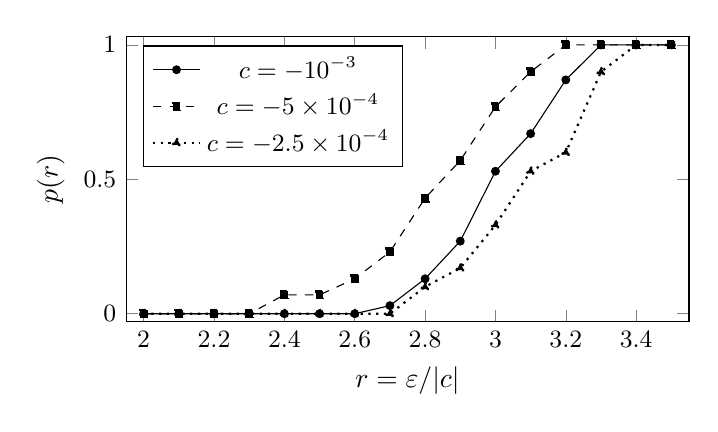
\begin{tikzpicture}
\begin{axis}[width=0.72\textwidth,height=5.2cm,xlabel={$r=\eps/|c|$},ylabel={$p(r)$},
  xmin=1.95,xmax=3.55,ymin=-0.03,ymax=1.03,legend pos=north west,legend style={font=\small},
  tick label style={font=\small}]
\addplot[mark=*,mark size=1.4pt] coordinates {(2.0,0)(2.1,0)(2.2,0)(2.3,0)(2.4,0)(2.5,0)(2.6,0)(2.7,0.03)(2.8,0.13)(2.9,0.27)(3.0,0.53)(3.1,0.67)(3.2,0.87)(3.3,1)(3.4,1)(3.5,1)};
\addplot[mark=square*,mark size=1.4pt,dashed] coordinates {(2.0,0)(2.1,0)(2.2,0)(2.3,0)(2.4,0.07)(2.5,0.07)(2.6,0.13)(2.7,0.23)(2.8,0.43)(2.9,0.57)(3.0,0.77)(3.1,0.90)(3.2,1)(3.3,1)(3.4,1)(3.5,1)};
\addplot[mark=triangle*,mark size=1.6pt,dotted,thick] coordinates {(2.0,0)(2.1,0)(2.2,0)(2.3,0)(2.4,0)(2.5,0)(2.6,0)(2.7,0)(2.8,0.10)(2.9,0.17)(3.0,0.33)(3.1,0.53)(3.2,0.60)(3.3,0.90)(3.4,1)(3.5,1)};
\legend{$c=-10^{-3}$,$c=-5\times10^{-4}$,$c=-2.5\times10^{-4}$}
\end{axis}
\end{tikzpicture}
\caption{Fraction of thirty equally spaced starting angles $\beta\in[0.40,0.52]$ for which the second
Fibonacci transition breaks, against $r=\eps/|c|$, every disk of diameter~\eqref{eq:diam}. For these sampled rates, angles and ratios, $p=0$ at $r\le2.3$ and $p=1$ at
$r\ge3.4$; values between grid points are not asserted.}\label{fig:pr}
\end{figure}

A heuristic decomposition of the crossover follows the mechanism of Section~\ref{sec:steptwo}. The pentagon fits when the
inherited mismatch $\theta=|\eps|-\kappa_1|c|$ exceeds the cushion $\sigma$ plus $\kappa_2|c|$ (Lemma~\ref{lem:pent}),
so the break happens near
\[
\frac{|\eps|}{|c|}\approx\kappa_1+\kappa_2+\frac{\sigma}{|c|}.
\]
With $\kappa_1\approx1.40$ and $\kappa_2\approx1.26$ at $\beta=0.523$, and $\sigma/|c|$ between about $-0.4$
and $0.7$ depending on the overshoot $\delta$ in~\eqref{eq:cushion}, which is set by where the discrete steps
fall when the hinge crosses $120^\circ$, this gives $2.3$ to $3.4$, consistent with the band. The spread
of the overshoot is what keeps $K^*$ from being sharp.

\begin{table}[h]
\centering\small
\begin{tabular}{@{}lccccc@{}}
\toprule
$\beta$ & $0.42$ & $0.45$ & $0.48$ & $0.50$ & $0.523$\\
\midrule
$\kappa_1=(\eps-\theta)/|c|$ & $1.665$ & $1.622$ & $1.568$ & $1.518$ & $1.399$\\
\bottomrule
\end{tabular}
\caption{The $O(c)$ loss of mismatch through the first transition, every disk of
diameter~\eqref{eq:diam}, stable to three digits over $c\in\{-2,-1,-0.5\}\times10^{-3}$ and
$\eps/|c|\in\{5,8\}$ (\texttt{verify/kappa1\_consistent.py}). It depends on the seed convention: with a
common initial diameter it runs from $1.584$ to $1.657$, increasing in $\beta$.}\label{tab:kappa1}
\end{table}

Two supplementary checks support the simulations, with limited scope. A second implementation, written independently (bisection for the
implicit diameter, overlap tests against all disks of the last 400 steps), reproduces the same events step
for step, including the pentagon at $(3,4)\to(3,3)$. Tolerance comparisons between $0$ and $10^{-7}$ leave the tested event histories unchanged
(\texttt{verify/independent\_tolerance.out}); this is a finite reproducibility check. The
400-step overlap window is a truncation in that implementation, not a proved global bound. The lattice starts ($\eps=0$) generate their own irregularity of about $0.16$ to $0.6$ times
$|c|$, below $K^*$, which is consistent with the Fibonacci transitions observed from regular fronts
in the small-rate sweeps of~\cite{GDD}.

\section{Discussion}\label{sec:discussion}

Theorem~\ref{thm:static} rules out a uniform initial Fibonacci guarantee based on three
independent upper bounds. It identifies the competing local scales and gives explicit
fronts realising a first pentagon. It does not show that a mismatch-to-rate bound is necessary
or sufficient for every front. The cancellation estimate explains persistence of a mismatch
within a rhombic phase; it does not by itself determine which transition ends that phase.
For the three-disk family, the numerical evidence motivates the following narrower statement.

\begin{quote}
\emph{Conjecture.} For every compact set of $\beta\in(\beta_{\min},\pi/6)$ there are $K>0$, $\eps_0>0$ and
$c_0>0$ such that for $0<|c|<c_0$ and $|\eps|<\min(\eps_0,K|c|)$, stacking from $F(\beta,\eps)$ completes the
first two Fibonacci transitions.
\end{quote}

\noindent Together with Conjecture~\ref{thm:B}, if both were proved, this would identify $|\eps|/|c|$ as the controlling parameter of the
second transition, with the simulations putting the crossover between about $2$ and $3.5$. For general
fronts we only ask: do fronts of parastichy numbers $(m,n)$ with $J\le |c|/K$ and notch angles
in a compact subset of $(60^\circ,120^\circ)$ undergo $N$ Fibonacci transitions, for $K$ large and $|c|$
small? Other open questions: a complete certificate for Conjecture~\ref{thm:B}, including zero-clearance branches;
whether breakdown always precedes $(3,5)$, as the sampled runs indicate; a closed form for
$\kappa_1$, the accumulated first-order residue of Proposition~\ref{prop:frozen} through the first
transition; whether a sharp threshold exists in a scaling limit that averages the overshoot; explicit
$\eps_0$ and $K$ for a proved delayed-breakdown statement; and the relation to the noise experiments of
Swinton~\cite{Swinton2024}, where irregularity is renewed at every disk instead of being inherited once.

The biological interpretation is limited to this model. Its local geometry shows that slowing
the diameter decrease reduces the clearance created at a transition. Relating this sensitivity
to measured growth rates or sunflower defects would require a calibrated model and data beyond
the computations reported here.

\appendix
\section{Formal verification}\label{app:lean}

The accompanying Lean~4 project specifies toolchain v4.34.0 and Mathlib. Its files verify the
statements identified below, using the standard axioms
(\texttt{propext}, \texttt{Classical.choice}, \texttt{Quot.sound}). Rechecking a file establishes its encoded statement; equivalence
to the geometric model still requires the hypotheses and scope described here.

\begin{center}\small
\begin{tabular}{@{}>{\raggedright\arraybackslash}p{0.36\textwidth}>{\raggedright\arraybackslash}p{0.2\textwidth}>{\raggedright\arraybackslash}p{0.38\textwidth}@{}}
\toprule
Result & Lean file & main theorems\\
\midrule
Lemma~\ref{lem:threshold}, $K_0$, Lemma~\ref{lem:K0} identities, $\sqrt{3/28}$ & \lean{Tilings} & \lean{threshold\_tan}, \lean{K0.height\_gaps}\\
Lemmas~\ref{lem:notch60}, \ref{lem:hexsite} (at $Q_0$), \ref{lem:hexclear}, \ref{lem:valid} (notch); $\mu_Z>0$ on valid fronts & \lean{Static} & \lean{notch60\_tan}, \lean{lattice\_Q0}, \lean{pentagon\_first}, \lean{notch\_clear}, \lean{channel\_of\_valid}\\
Local five-disk families: hypotheses satisfiable & \lean{StaticExists} & \lean{front\_exists}\\
Lemma~\ref{lem:apex}: differentiability at $0$, tangency nearby and local uniqueness (not the full $C^1$ neighbourhood statement); non-vacuity & \lean{Apex}, \lean{Lemma4Exists} & \lean{apex\_exists}, \lean{rhombic\_family\_exists}\\
Lemmas~\ref{lem:rhombus}, \ref{lem:triangle}, Corollary~\ref{cor:rates} & \lean{FirstOrder} & \lean{rhombic\_step}, \lean{triangle\_step}, \lean{cushion\_rate}\\
Margin~\eqref{eq:ddu} and $\sqrt7$ & \lean{FirstOrder}, \lean{Lemma4} & \lean{split\_rate}, \lean{pass\_rate}, \lean{n1\_exclusion}\\
Lemma~\ref{lem:pent} & \lean{Lemma4} & \lean{dG\_dc}, \lean{dG\_d$\theta$}, \lean{kappa2\_eq}, \lean{boundary\_slope}\\
Lemma~\ref{lem:passes}, gap in Lemma~\ref{lem:alternation} & \lean{PassBalance}, \lean{Sweep} & \lean{pass\_balance}, \lean{pass\_lag}, \lean{sweep}, \lean{alternation\_gap}\\
Proposition~\ref{prop:frozen} & \lean{Prop2} & \lean{prop2}\\
\bottomrule
\end{tabular}
\end{center}

The local existence results in \lean{Apex} and \lean{StaticExists} do not certify periodic
closure or global placement order. The following steps are proved by hand and remain outside
Lean: the uniform remainders (Lemma~\ref{lem:uniform}); the full periodic first-disk argument,
namely the ridge clearance (Lemma~\ref{lem:valid}), the lattice order (Lemma~\ref{lem:hexsite}), the
separation of $Z$ and $E$, and the exclusion of all other positions (proof of
Theorem~\ref{thm:static}). Also outside Lean are the rational candidate enumerations; and the lattice-order argument in
Lemma~\ref{lem:32phase}. The first-order burst exploration is also outside Lean and, as
explained in Section~\ref{sec:burst}, does not yet prove Conjecture~\ref{thm:B}.

\section*{Data and code availability}
The simulators, recorded outputs, exact enumerations, first-order burst calculation and Lean source
files are at~\cite{repo}, with a snapshot identifying the revision. The README there distinguishes
reproduced checks from supplied records and lists the open proof obligations.

\section*{Acknowledgements}
Two AI systems were used in this work under the author's direction. Claude Opus 5.5 (Anthropic)
developed the simulations, the first-order analysis and its proofs, the Lean formalisation and the
draft. Codex (OpenAI, GPT-6) reviewed the draft, found an earlier first-disk pentagon on a
five-disk front with one directional deviation zero, which prompted the construction of
Theorem~\ref{thm:static} on a different family of fronts, and contributed the revision that
recast delayed breakdown as Conjecture~\ref{thm:B}, computational checks and the identification of
proof obligations. In version 2, a Codex referee report found the gap in the proof of
Theorem~\ref{thm:A} described below; Codex proved Lemma~\ref{lem:shared} and the strict bound for the words
$\Ua\,\dn{\Ub}\,D\,\up{\Ub}$ and $\Ua\,D\,\dn{\Ub}\,\up{\Ub}$, including the treatment of the triple
$D,\dn{\Ub},\up{\Ub}$, and Claude checked both against independent simulations and an independent
derivation of the same comparison. The author is responsible for the content of this preprint, which has not yet
been independently reviewed.

\emph{Changes in version 2.} Version 1 asserted that the first triangle wins by an order-one margin and
that the only near-tie in the $(2,2)$ phase is the second triangle. Both are wrong: at each triangle
event, and in two of the four words of the $(2,2)$ phase, a triangle on a down vector coincides with the
intended placement at the threshold tiling, and one two-down triple was not treated. Lemma~\ref{lem:shared}
and the margin~\eqref{eq:dud} close the gap, and Theorem~\ref{thm:A} stands as stated. The triangle
threshold is $120^\circ+O(|c|)$, not exactly $120^\circ$ (Section~\ref{sec:stepone}, Lemma~\ref{lem:32phase});
the first-disk theorem is stated for single-notch fronts $D^mU^n$; Swinton's version and sections are
cited; the Lean coverage of Lemma~\ref{lem:apex} is stated exactly; the recorded outputs and the
verification scripts are completed and every script exits nonzero on a failure.

\begin{thebibliography}{99}
\bibitem{repo} V.~Jandhyala, \emph{Irregularity versus growth rate in disk-stacking phyllotaxis: code, records and Lean
sources}, \url{https://github.com/jvvk/mathematics/tree/main/phyllotaxis-irregularity}.
\bibitem{AGH} P.~Atela, C.~Gol\'e and S.~Hotton, \emph{A dynamical system for plant pattern formation: a
rigorous analysis}, J.\ Nonlinear Sci.\ \textbf{12} (2002), no.~6, 641--676.
\href{https://doi.org/10.1007/s00332-002-0513-1}{doi:10.1007/s00332-002-0513-1}.
\bibitem{AtelaGole} P.~Atela and C.~Gol\'e, \emph{Rhombic tilings and primordia fronts of phyllotaxis},
preprint (2017), \href{https://arxiv.org/abs/1701.01361}{arXiv:1701.01361}.
\bibitem{DouadyCouder} S.~Douady and Y.~Couder, \emph{Phyllotaxis as a physical self-organized growth
process}, Phys.\ Rev.\ Lett.\ \textbf{68} (1992), no.~13, 2098--2101.
\href{https://doi.org/10.1103/PhysRevLett.68.2098}{doi:10.1103/PhysRevLett.68.2098}.
\bibitem{GD} C.~Gol\'e and S.~Douady, \emph{Convergence in a disk stacking model on the cylinder},
Phys.\ D \textbf{403} (2020), 132278.
\href{https://doi.org/10.1016/j.physd.2019.132278}{doi:10.1016/j.physd.2019.132278}.
\bibitem{GDD} C.~Gol\'e, J.~Dumais and S.~Douady, \emph{Fibonacci or quasi-symmetric phyllotaxis. Part I:
why?}, Acta Soc.\ Bot.\ Pol.\ \textbf{85} (2016), no.~4, 3533.
\href{https://doi.org/10.5586/asbp.3533}{doi:10.5586/asbp.3533}.
\bibitem{Lean4} L.~de Moura and S.~Ullrich, \emph{The Lean 4 theorem prover and programming language},
in: Automated Deduction, CADE 28, Lecture Notes in Comput.\ Sci.\ \textbf{12699}, Springer, 2021, 625--635.
\href{https://doi.org/10.1007/978-3-030-79876-5_37}{doi:10.1007/978-3-030-79876-5\_37}.
\bibitem{Mathlib} The mathlib Community, \emph{The Lean mathematical library}, in: Proceedings of the 9th
ACM SIGPLAN International Conference on Certified Programs and Proofs (CPP 2020), 367--381.
\href{https://doi.org/10.1145/3372885.3373824}{doi:10.1145/3372885.3373824}.
\bibitem{Schwendener} S.~Schwendener, \emph{Mechanische Theorie der Blattstellungen}, Engelmann, Leipzig, 1878.
\bibitem{Swinton2024} J.~Swinton, \emph{Disk-stacking models are consistent with Fibonacci and non-Fibonacci
structure in sunflowers}, preprint, version 3 (2 September 2024),
\href{https://arxiv.org/abs/2407.05857v3}{arXiv:2407.05857v3}.
\bibitem{SwintonOchu} J.~Swinton, E.~Ochu and the MSI Turing's Sunflower Consortium, \emph{Novel Fibonacci
and non-Fibonacci structure in the sunflower: results of a citizen science experiment}, R.\ Soc.\ Open
Sci.\ \textbf{3} (2016), no.~5, 160091.
\href{https://doi.org/10.1098/rsos.160091}{doi:10.1098/rsos.160091}.
\end{thebibliography}
\end{document}
